\documentclass[]{scrreprt}

% Лицензия
% Apache License Version 2.0, January 2004
% http://www.apache.org/licenses/
% Copyright [2020] [Kirill A. Murashev]
% Licensed under the Apache License, Version 2.0 (the "License"); you may not use this file except in compliance with the License. You may obtain a copy of the License at
% http://www.apache.org/licenses/LICENSE-2.0
% Unless required by applicable law or agreed to in writing, software
% distributed under the License is distributed on an "AS IS" BASIS,
% WITHOUT WARRANTIES OR CONDITIONS OF ANY KIND, either express or implied.
% See the License for the specific language governing permissions and limitations under the License.


%%% Работа с русским языком
\usepackage{cmap}					% поиск в PDF
\usepackage{mathtext} 				% русские буквы в формулах
\usepackage{fontspec}
\defaultfontfeatures{Renderer=Basic,Ligatures={TeX}}
\setmainfont{CMU Serif}
\setsansfont{CMU Sans Serif}
\setmonofont{CMU Typewriter Text}
\usepackage[english,russian]{babel}
%\usepackage[T1,T2A]{fontenc}			% кодировка
%\usepackage[lutf8]{luainputenc}			% кодировка исходного текста
%\usepackage[english,russian]{babel}	% локализация и переносы
\usepackage{indentfirst}            % красная строка
\usepackage{misccorr}               % доработки для babel
\frenchspacing                      % французский стиль пробелов

%\usepackage{beton} %изменение шрифта для тёмной цветовой схемы
%\usepackage{concrete}
%%% Дополнительная работа с математикой
\usepackage{amsmath,amsfonts,amssymb,amsthm,mathtools} % AMS
\usepackage{icomma} % "Умная" запятая: $0,2$ --- число, $0, 2$ --- перечисление

%% Номера формул
%\mathtoolsset{showonlyrefs=true} % Показывать номера только у тех формул, на которые есть \eqref{} в тексте.
%\usepackage{leqno} % Нумерация формул слева

%% Перенос знаков в формулах (по Львовскому)
\newcommand*{\hm}[1]{#1\nobreak\discretionary{}
	{\hbox{$\mathsurround=0pt #1$}}{}}

%%% Работа с картинками
\usepackage{graphicx}  % Для вставки рисунков
\graphicspath{{Images/}}  % папки с картинками
\setlength\fboxsep{3pt} % Отступ рамки \fbox{} от рисунка
\setlength\fboxrule{1pt} % Толщина линий рамки \fbox{}
\usepackage{wrapfig} % Обтекание рисунков текстом

%%% Работа с таблицами
\usepackage{array, tabularx, tabulary, booktabs, xtab} % Дополнительная работа с таблицами
\usepackage{longtable}  % Длинные таблицы
\usepackage{multirow} % Слияние строк в таблице

%%% Теоремы
\theoremstyle{plain} % Это стиль по умолчанию, его можно не переопределять.
\newtheorem{theorem}{Теорема}[section]
\newtheorem{proposition}[theorem]{Утверждение}
\newtheorem{lemma}[theorem]{Лемма}

\theoremstyle{definition} % "Определение"
\newtheorem{corollary}{Следствие}[theorem]
\newtheorem{problem}{Задача}[section]

\theoremstyle{remark} % "Примечание"
\newtheorem*{nonum}{Решение}

%%% Программирование
\usepackage{etoolbox} % логические операторы

\usepackage{lastpage} % Узнать, сколько всего страниц в документе.

\usepackage{keyval}

\usepackage{totcount} % Узнать, сколько всего объектов в документе.

%\usepackage{xcolor-solarized}

%%% Страница
%\usepackage{extsizes} % Возможность сделать 14-й шрифт
%\usepackage{geometry} % Простой способ задавать поля
%	\geometry{top=25mm}
%	\geometry{bottom=35mm}
%	\geometry{left=35mm}
%	\geometry{right=20mm}
%

%\usepackage{fancyhdr} % Колонтитулы

%	\pagestyle{fancy}
%\renewcommand{\headrulewidth}{0pt}  % Толщина линейки, отчеркивающей верхний колонтитул
%\fancyhf{}
%\lhead{Часть \thepart}
%\chead{Глава \thechapter}
%\rhead{Раздел \thesection}
%\lfoot{version 0.251}
%\cfoot{\today} % По умолчанию здесь номер страницы
%\rfoot{\thepage/\ref{LastPage}}
%\pagestyle{fancy}

%\usepackage{setspace} % Интерлиньяж
%\onehalfspacing % Интерлиньяж 1.5
%\doublespacing % Интерлиньяж 2
%\singlespacing % Интерлиньяж 1

\usepackage{soul} % Модификаторы начертания

\usepackage[usenames,dvipsnames,svgnames,table,rgb]{xcolor} % Подключение пакета для задания цвета

%\definecolor{Backcolor}{HTML}{042029} % Задание цвета для фона
%\definecolor{Textcolor}{HTML}{819090} % Задание цвета для текста
%\pagecolor{Backcolor}                 % Подключение тёмной
%\color{Textcolor}                     % темы

\usepackage{csquotes} % Ещё инструменты для ссылок

\usepackage[backend=biber,bibencoding=utf8,sorting=ynt,maxcitenames=5,sortupper=true,date=iso]{biblatex} % подключение пакета для работы с автоматизированной библиографией

%\usepackage[style=authoryear,maxcitenames=2,backend=biber,sorting=nty]{biblatex}

%\renewcommand\bibname{Источники информации} % Переопределение названия для библиографии

\usepackage{multicol} % Несколько колонок

\usepackage{microtype}              %<-- added for better inter word spacing

\usepackage{tabularx}

\usepackage{tikz} % Работа с графикой
\usepackage{pgfplots}
\usepackage{pgfplotstable}

\usepackage{eqlist}

\usepackage{desclist} % Дополнительное окружение для списка Глоссария

\setcounter{tocdepth}{8} % Глубина оглавления

% подавление висячих строк
\clubpenalty=400 % Разрешение = 300, абсолютный запрет = 10000
\widowpenalty=400 % Увеличиваем эти числа до тех пор, пока не начнёт увеличиваться количество страниц.

% Выбор между разрежением и переполнением
\tolerance=500 % max=10000, default=200

\looseness=-1 % иногда можно удлинять страницу на одну строку.

\hfuzz=2.5pt % иногда можно вылезти за край строки на 2.5 pt.

\usepackage{calc} % Вычисления

\usepackage{scrlayer-scrpage} % Стиль страницы

\usepackage{lineno} % нумерация строк

%\pagestyle{scrpage}

%\usepackage{concrete}

\usepackage{booktabs}

\usepackage[owncaptions]{vhistory} % Log of versions

\usepackage{progressbar} % Формирование линейки, показывающей прогресс в работе

\usepackage{epigraph} % работа с эпиграфами

\usepackage {listings}
\lstloadlanguages{[Latex]Tex, bash, R, Python, SQL}
\lstset{extendedchars=true , % включаем не латиницу
frame=tb, % рамка сверху и снизу
commentstyle=\itshape , % шрифт для комментариев
stringstyle =\ttfamily % шрифт для строк
keywordstyle=\color{blue}
}

%\usepackage{titling} %дополнительная настройка титульного листа

\setcounter{secnumdepth}{8} % Установка глубины нумерации заголовков

% Работа с гиперрсылками, подключается последним
\usepackage{hyperref}       % Подключение пакета для работы с гиперссылками
\hypersetup{				% Гиперссылки
	unicode=true,           % русские буквы в раздела PDF
	pdftitle={Искусственный интеллект в~оценке стоимости},   % Заголовок
	pdfauthor={К.\,А.~Мурашев},      % Автор
	pdfsubject={Системы поддержки принятия решений, основанные на искусственном интеллекте},      % Тема
	pdfcreator={К.\,А.~Мурашев}, % Создатель
	pdfproducer={К.\,А.~Мурашев}, % Производитель
	pdfkeywords={Искусственный интеллект, машинное обучение, математические методы, оценочная деятельность, цифровая экономика, Data Science, анализ данных} % Ключевые слова
	colorlinks=true,       	% false: ссылки в рамках; true: цветные ссылки
	linkcolor=red,          % внутренние ссылки
	citecolor=green,        % на библиографию
	filecolor=magenta,      % на файлы
	urlcolor=blue           % на URL
}

\usepackage{pgfplots} 
\pgfplotsset{compat=1.15}
\usepackage{mathrsfs}
\usetikzlibrary{arrows}
%\usepackage{url}

%\usepackage{totpages}

%\usepackage[strings]{underscore}

%\author{К.\,А.~Мурашев\thanks {\href{kirill.murashev@tutanota.de}{kirill.murashev@tutanota.de}, \href{https://t.me/Maas\_88}{https://t.me/Maas\_88}, \href{https://www.facebook.com/murashev.kirill}{https://www.facebook.com/murashev.kirill}}}
%\title{\Large Современные системы поддержки принятия решений оценщиками, основанные на~применении методов машинного обучения: практическое руководство по~применению языка программирования R в~повседневной практике оценщика}
%\date{\today}

%\normalsize

% Макрос для рисунков, обтекаемых текстом
\newcommand*{\EpsWrapD}[7]{%
	\begin{wrapfigure}[#5]{#3}{#2 \textwidth} % #3=l,r,L,R
		\begin{center} \sffamily
			\includegraphics*[width= #2 \textwidth ]{#1} % 1-имя файла и метка заодно,
			% 2-ширина рисунка (доля от ширины страницы)
			\vspace{-#7mm} % #7: сократить расстояние между подписью снизу и рисунком
			\caption{\label{fig:#1}#4} % #4 - подпись под рисунком
			\vspace{-#6pt}
		\end{center}% #6: сократить расстояние между подписью снизу и текстом после таблицы 
	\end{wrapfigure}}
%
% макрос для создания таблицы, обтекаемой текстом
\newcommand*{\TableBE}[5]{
	\begin{table}[#1] %\captionabove
		\vspace*{-#5mm}
		\centering \sffamily \caption{\label{tab:#2}#3} \begin{tabular}{#4} \toprule }
		
		\newcommand*{\TableEN}[3]{
			\bottomrule \end{tabular}
		\vspace{-#2mm} \small \begin{flushleft} #1 \end{flushleft}
		\vspace{-#3mm}
\end{table}}


\addbibresource{/home/kaarlahti/TresoritDrive/Methodics/My/AI_for_valuers/Book/AI_for_valuers_book/Basic_principles.bib}
\addbibresource{/home/kaarlahti/TresoritDrive/Methodics/My/AI_for_valuers/Book/AI_for_valuers_book/LaTeX.bib}
\addbibresource{/home/kaarlahti/TresoritDrive/Methodics/My/AI_for_valuers/Book/AI_for_valuers_book/Mathstat.bib}
\addbibresource{/home/kaarlahti/TresoritDrive/Methodics/My/AI_for_valuers/Book/AI_for_valuers_book/Murashev.bib}
\addbibresource{/home/kaarlahti/TresoritDrive/Methodics/My/AI_for_valuers/Book/AI_for_valuers_book/Python.bib}
\addbibresource{/home/kaarlahti/TresoritDrive/Methodics/My/AI_for_valuers/Book/AI_for_valuers_book/R.bib}
\addbibresource{/home/kaarlahti/TresoritDrive/Methodics/My/AI_for_valuers/Book/AI_for_valuers_book/RussianLaws.bib}
\addbibresource{/home/kaarlahti/TresoritDrive/Methodics/My/AI_for_valuers/Book/AI_for_valuers_book/Sci&Tech.bib}
\addbibresource{/home/kaarlahti/TresoritDrive/Methodics/My/AI_for_valuers/Book/AI_for_valuers_book/Valuation.bib}
\addbibresource{/home/kaarlahti/TresoritDrive/Methodics/My/AI_for_valuers/Book/AI_for_valuers_book/ValuationStandards.bib}
\addbibresource{/home/kaarlahti/TresoritDrive/Methodics/My/AI_for_valuers/Book/AI_for_valuers_book/ZHZL.bib}

\pagestyle{headings} 
\markright{Искусственный интеллект в~оценке стоимости}
\usepackage{pgfplots}
\pgfplotsset{compat=1.15}
\usepackage{mathrsfs}
\usetikzlibrary{arrows}

%\usepackage{polyglossia}

%\usepackage{minted}

\newtheorem{Thexmpl}[theorem]{Пример}

\usepackage[inkscapearea=page]{svg}
\usepackage{adjustbox}

\DeclareMathOperator{\rank}{rank}
\makeatletter
\newenvironment{sqcases}{%
	\matrix@check\sqcases\env@sqcases
}{%
	\endarray\right.%
}
\def\env@sqcases{%
	\let\@ifnextchar\new@ifnextchar
	\left\lbrack
	\def\arraystretch{1.2}%
	\array{@{}l@{\quad}l@{}}%
}
\makeatother

\DeclareMathOperator{\arcsec}{arcsec}
\DeclareMathOperator{\arccot}{arccot}
\DeclareMathOperator{\arccsc}{arccsc}
\DeclareMathOperator{\sgn}{sgn}

\renewcaptionname{russian}{\listfigurename}{Список диаграмм}
%\renewcommand{russian}{\lstlistingname}{Скрипт}

%\definecolor{deepblue}{rgb}{0,0,0.5}
%\definecolor{deepred}{rgb}{0.6,0,0}
%\definecolor{deepgreen}{rgb}{0,0.5,0}

% Python style for highlighting
%\newcommand\pythonstyle{\lstset{
%language=Python,
%basicstyle=\ttm,
%morekeywords={self},              % Add keywords here
%keywordstyle=\ttb\color{deepblue},
%emph={MyClass,__init__},          % Custom highlighting
%emphstyle=\ttb\color{deepred},    % Custom highlighting style
%stringstyle=\color{deepgreen},
%frame=tb,                         % Any extra options here
%showstringspaces=false
%}}

% Python environment
%\lstnewenvironment{python}[1][]
%{
%\pythonstyle
%\lstset{#1}
%}
%{}

% Python for external files
%\newcommand\pythonexternal[2][]{{
%\pythonstyle
%\lstinputlisting[#1]{#2%}%}%}

% Python for inline
%\newcommand\pythoninline[1]{{\pythonstyle\lstinline!#1!}}



%opening
\title{Практическое применение критерия Манна--~Уитни--~Уилкоксона в~оценочной деятельности}

\author{\href{https://www.facebook.com/murashev.kirill/}{K.\,A.~{Мурашев}}}

\begin{document}
	
\maketitle


	
\begin{abstract}
	В~своей практике оценщики часто сталкиваются с~необходимостью учёта различий количественных характеристик объектов. В~частности, одной из~стандартных задач является установление признаков, влияющих на~стоимость~(т.\,н.~ценообразующих факторов) и~их~отделение от~признаков, влияние которых на~стоимость отсутствует либо не~может быть установлено.
	
	В~практике оценки широкое распространение получил субъективный отбор признаков, учитываемых при~определении стоимости. При~этом конкретные количественные показатели влияния этих признаков на~стоимость зачастую берутся из~т.\,н.~<<справочников>>. Не~отказывая такому подходу в~быстроте и~невысокой стоимости его~реализации, нельзя не~признать, что~только данные, непосредственно наблюдаемые на~открытом рынке, являются надёжной основой суждения о~стоимости. Приоритет таких данных над~прочими, в~частности, полученными путём опроса экспертов, закреплён, в~том~числе в~\href{https://www.rics.org/uk/upholding-professional-standards/sector-standards/valuation/red-book/red-book-global/}{Стандартах оценки~RICS}~\cite{RVGS-2022}, \href{https://www.rics.org/uk/upholding-professional-standards/sector-standards/valuation/red-book/international-valuation-standards/}{Международных стандартах оценки~2022}~\cite{IVS-2022}, а~также в~ \href{https://normativ.kontur.ru/document?moduleId=1&documentId=326168#l0}{МСФО~13~<<Оценка справедливой стоимости}~\cite{MSFO-13}. Поэтому можно говорить о~том, что~математические методы анализа данных, полученных на~открытом рынке, являются наиболее надёжным средством интерпретации рыночной информации, применяемой при~исследованиях рынка и~предсказании стоимости конкретных объектов.
	
		Основной материал состоит из~четырёх блоков:
\begin{itemize}
	\item описание теста Манна"--~Уитни"--~Уилкоксона~(далее \emph{U-тест}), его~вероятностного смысла и~связи с~другими математическими методами;
	\item практическая реализация U-теста в~электронной таблице на~примере тестовых случайных данных;
	\item практическая реализация U-теста на~реальных данных рынка жилой недвижимости Санкт-Петербургской агломерации средствами языка программирования Python, целью анализа являлась проверка существенности различия удельной стоимости между объектами, расположенными в~городской и~пригородной частях агломерации;
	\item практическая реализация U-теста на~реальных данных рынка жилой недвижимости города Алматы средствами языка программирования R, целью анализа являлась проверка существенности различия удельной стоимости между объектами, продаваемыми без~отделимых улучшений и~объектами, продаваемыми вместе с~ними.
\end{itemize}
	Актуальная версия данного материала, её~исходный код, скрипты на~Python и~R, а~также электронная таблица находятся в~репозитории на~портале GitHub и~доступны по~\href{https://github.com/Kirill-Murashev/AI_for_valuers_book/tree/main/Parts-Chapters/Mann-Whitney-Wilcoxon}{постоянной ссылке}~\cite{Murashev:u-test}.
	
	Данный материал и~все~приложения к~нему распространяются на~условиях лицензии \href{https://creativecommons.org/licenses/by-sa/4.0/}{cc-by-sa-4.0}~\cite{cc-by-sa-4.0}.
\end{abstract}
%
\tableofcontents
\listoftables
\listoffigures
\lstlistoflistings
%
\chapter{Технические данные}
Данный материал, а~также приложения к~нему доступны по~\href{https://github.com/Kirill-Murashev/AI_for_valuers_book/tree/main/Parts-Chapters/Mann-Whitney-Wilcoxon}{постоянной ссылке}~\cite{Murashev:u-test}. Исходный код данной работы был~создан с~использованием языка~\href{https://www.ctan.org/}{\TeX}~\cite{TeX:site} c~набором макрорасширений~\href{https://www.latex-project.org/}{\LaTeXe}~\cite{LaTeX:site}, дистрибутива~\href{https://www.tug.org/texlive/}{TeXLive}~\cite{TeXLive:site} и~редактора~\href{https://www.texstudio.org/}{TeXstudio}~\cite{TeXstudio:site}. Расчёт в~форме электронной таблицы был выполнен с~помощью \href{https://www.libreoffice.org/discover/calc/}{LibreOffice Calc}~\cite{LO:Calc} (Version: 7.3.3.2, Ubuntu package version: 1:7.3.3~rc2-0ubuntu0.20.04.1~lo1 Calc: threaded). Расчёт на~языке~\href{https://www.r-project.org/}{R}~\cite{R_language} (version 4.2.0 (2022-04-22) -- "Vigorous Calisthenics") был выполнен c~использованием IDE~\href{https://www.rstudio.com/}{RStudio} (RStudio 2022.02.2+485 "Prairie Trillium" Release (8acbd38b0d4ca3c86c570cf4112a8180c48cc6fb, 2022-04-19) for Ubuntu Bionic Mozilla/5.0 (X11; Linux x86\_64) AppleWebKit/537.36 (KHTML, like Gecko) QtWebEngine/5.12.8 Chrome/69.0.3497.128 Safari/537.36)~\cite{RStudio:official_site}. Расчёт на~языке \href{https://www.python.org/}{Python}~(Version~3.9.12)~\cite{Python:site} был выполнен с~использованием среды разработки \href{https://jupyter.org}{Jupyter Lab} (Version 3.4.2)~\cite{Jupyter:site} и~IDE \href{https://www.spyder-ide.org/}{Spyder} (Spyder version: 5.1.5 None* Python version: 3.9.12 64-bit * Qt version: 5.9.7 * PyQt5 version: 5.9.2
* Operating System: Linux 5.11.0-37-generic)~\cite{Spyder:site}. Графические материалы, использованные в~подсекции~\ref{U-test-spreadsheet}, были подготовлены с~использованием~\href{Geogebra:official-site}{Geogebra}~(Version 6.0.666.0-202109211234)~\cite{Geogebra:official-site}.
В~данном материале как~и~в~большинстве работ цикла были использованы следующие значения:
\begin{itemize}
	\item уровень значимости "--- $\alpha = 0.05$;
	\item доверительный интервал "--- $Pr = 0.95$;
	\item начальное положение датчика псевдослучайных чисел "--- $seed = 19190709$.
\end{itemize}
В~качестве десятичного знака используется точка. Большинство математических обозначений записаны так, как~это принято в~англоязычной среде. Например, тангенс обозначается как~$\tan$, а~не~$\tg$. Результаты статистических тестов признаются значимыми в~случае, когда
\begin{equation}\label{eq:ignificance }
 p \leq \alpha.
\end{equation}
Данное решение основано, в~частности на~результатах\href{researchgate.net}{дискуссии}, имевшей место на~портале researchgate.net~\cite{RG:p-equals-alpha}.
%
\chapter{Предмет исследования}
В~случае работы с~рыночными данными перед оценщиком часто встаёт задача проверки гипотезы о~существенности влияния на~стоимость того или~иного признака, измеренного в~количественной или~порядковой шкале. Аналогичная задача возникает у~аналитиков рынка недвижимости, специалистов компаний-застройщиков, риелторов. При~этом, зачастую отсутствует возможность сбора больших массивов данных, позволяющих применить широкий спектр методов машинного обучения. В~ряде случаев оценщики осознанно сужают область сбора данных до~узкого сегмента рынка, в~результате чего в~их~распоряжении оказываются лишь сверхмалые выборки объёмом менее тридцати наблюдений. При~этом, ценовые данные чаще всего имеют распределение отличное от~нормального. В~данном случае рациональным решением является применение U-теста. Сформулируем задачу:
\begin{itemize}
	\item предположим, что~у~нас~существуют две~выборки удельных цен коммерческих помещений, часть из~которых обладает некоторым признаком (например, имеет отдельный вход), часть "--- нет;
	\item необходимо установить: оказывает~ли наличие этого признака существенное влияние на~удельную стоимость недвижимости данного типа или~нет.
\end{itemize}
На~первый взгляд, согласно сложившейся практике, оценщик может просто субъективно признать те~или~иные признаки значимыми, а~прочие нет, после чего принять значения корректировок на~различия в~этих признаках из~справочников. Однако, как~было сказано выше, такой подход вряд~ли может считаться лучшей практикой, поскольку в~этом случае отсутствует какой-либо анализ рынка. Кроме того, в~таком случае вряд~ли можно говорить о~серьёзной ценности такой работы в~принципе.

Вместо этого возможно использовать случайные выборки рыночных данных и~применять к~ним математические методы анализа, позволяющие делать доказательные с~научной точки зрения выводы о~значимости влияния на~стоимость со~стороны того или~иного признака. Данные, используемые в~настоящей работе при~проведении U-теста средствами Python и~R, представляют собой реальные рыночные данные, часть из~которых была собрана автором путём веб-скрепинга, часть "--- предоставлена коллегами для~анализа. Прилагаемая электронная таблица настроена таким образом, что~тестовые исходные данные могут быть сгенерированы случайно.

\chapter{Основные сведения о~тесте}
\section{Предпосылки и~формализация гипотез}
В~первую очередь необходимо сказать, что, несмотря на~заявленное общее название, правильнее всё~же говорить о~двух тестах:
\begin{itemize}
	\item \href{http://www.machinelearning.ru/wiki/index.php?title=Критерий_Уилкоксона_двухвыборочный}{двухвыборочный критерий Уилкоксона}, разработанный Фрэнком Уилкоксоном в~1945~году~\cite{MLRU:Wilcoxon-test};
	\item \href{http://www.machinelearning.ru/wiki/index.php?title=Критерий_Уилкоксона-Манна"--~Уитни}{U-критерий Манна--~Уитни}, являющийся дальнейшим развитием вышеуказанном критерия, разработанный Генри Манном и~Дональдом Уитни в~1947~году~\cite{MLRU:Mann-Whitney}.
\end{itemize}
Забегая вперёд, можно сказать о~том, что~статистики данных критериев линейно связаны, а~их p-значения почти одинаковы, что~с~практической точки зрения позволяет говорить о~вариациях одного теста, а~не~о~двух отдельных~\cite{MLRU:Wilcoxon-test}. В~данной работе по~всему тексту используется общее название, а~также его~сокращённый вариант "--- U-тест, исторически относимый к~критерию Манна"--~Уитни. Некоторые авторы~\cite{Kobzarq-prikl-mathstat} рекомендуют использовать двухвыборочный критерий Уилкоксона в~случаях, когда нет~предположений о~дисперсиях, а~в~случае равных дисперсий применять U-критерий Манна"--~Уитни. Однако экспериментальные данные указывают, что~p-значения критериев Уилкоксона и~Манна"--~Уитни практически совпадают в~том~числе и~в~случае, когда дисперсии выборок существенно различаются~\cite{MLRU:Wilcoxon-test}. Придерживаясь принципа KISS~\cite{KISS-principle}, лежащего в~основе всего данного цикла публикаций, автор приходит к~выводу о~возможности применения единого подхода. 

Также следует помнить о~том, что~существует \href{http://www.machinelearning.ru/wiki/index.php?title=Критерий_Уилкоксона_для_связных_выборок}{Критерий Уилкоксона для связных выборок}~\cite{Wilcoxon-signed-rank-test}, представляющий собой отдельный тест, предназначенный для~анализа различий между связанными выборками, тогда как~рассматриваемый в~данной работе U-тест предназначен для~работы с~двумя независимыми выборками.

Предположим, что~заданы две~выборки:
\begin{equation*}
	x^{m} = (x_{1},x_{2},\ldots,x_{m}), x_{i} \in \mathbb{R};\quad y^{n} = (y_{1},y_{2},\ldots,y_{n}), y_{i} \in \mathbb{R} \quad: m \leq n.
\end{equation*}
 
\begin{itemize}
	\item Обе выборки являются простыми, объединённая выборка независима.
	\item Выборки взяты из~неизвестных непрерывных распределений \textit{F(x)} и~\textit{G(y)} соответственно.
\end{itemize}
 
\begin{description}
	\item[Простая выборка "---] это~случайная, однородная, независимая выборка. Эквивалентное определение: выборка ${\textstyle x^{m} = (x_{1},x_{2},\ldots,x_{m})}$ является простой, если значения~${\textstyle (x_{1},x_{2},\ldots,x_{m})}$ являются реализациями \textit{m} независимых одинаково распределённых случайных величин. Иными словами, отбор наблюдений является не~только случайным, но~и~не~предполагает наличие каких-либо специальных правил отбора (например, выбор каждого 10-го наблюдения).
\end{description}
\begin{description}
	\item[U-тест "---] это~непараметрический тест для~проверки нулевой гипотезы, заключающейся в~том, что~для~случайно выбранных из~двух выборок наблюдений ${\textstyle x \in X}$ и~${\textstyle y \in Y}$ вероятность того, что~\textit{x} больше \textit{y}, равна вероятности того, что~\textit{y} больше~\textit{x}. На~математической языке запись нулевой гипотезы выглядит следующим образом:
	\begin{equation}\label{eq:U-test-null-hypothesis}
	H_{0}:P\{x<y=\frac{1}{2}\}.
	\end{equation}
	Для~целостности теста требуется альтернативная гипотеза, которая заключается в~том, что~вероятность того, что~значение признака у~наблюдения из~выборки~\textit{X} превышает его~у~наблюдения из~выборки~\textit{Y}, отличается (в~большую или~меньшую сторону) от~вероятности того, что~значение признака у~наблюдения из~\textit{Y} превышает значение у~наблюдения из~\textit{X}. На~математическом языке запись альтернативной гипотезы выглядит следующим образом:
	\begin{equation}\label{eq:U-test-alt-hypothesis}
	H_{1}:P\{x<y\} \neq P\{y<x\} \vee P\{x<y\} + 0.5 \cdot P\{x=y\} \neq 0.5.
	\end{equation}
\end{description}
Согласно базовой концепции U-теста, при~справедливости нулевой гипотезы распределение двух выборок непрерывно, при~справедливости альтернативной распределение одной из~них стохастически больше распределения другой. При~этом, можно сформулировать целый ряд нулевых и~альтернативных гипотез, для~которых данный тест будет давать корректный результат. Его~самое широкое обобщение заключается в~следующих предположениях:
\begin{itemize}
	\item наблюдения в~обеих выборках независимы;
	\item тип данных является как~минимум ранговым, т.\,е.~в~отношении любых двух наблюдений можно сказать, какое из~них~больше;
	\item нулевая гипотеза предполагает, что~распределения двух выборок равны;
	\item альтернативная гипотеза предполагает, что~распределения двух выборок не~равны.
\end{itemize}
При~более строгом наборе допущений, чем~приведённые выше, например, в~случае допущения о~том, что~распределение двух выборок в~случае справедливости нулевой гипотезы непрерывно, альтернативной "--- имеет сдвиг расположения двух распределений, т.\,е.~$f_{1}{x}=f_{2}(x+\sigma)$, можно сказать, что~U-тест представляет собой тест на~проверку гипотезы о~равенстве медиан. В~этом случае, U-тест можно интерпретировать как~проверку того, отличается~ли от~нуля оценка Ходжеса"--~Лемана разницы значений мер центральной тенденции. В~данной ситуации оценка Ходжеса"--~Лемана представляет собой медиану всех возможных значений различий между наблюдениями в~первой и~второй выборках. Вместе с~тем, если и~дисперсии, и~формы распределения обеих выборок различаются, U-тест не~может корректно проверить медианы. Можно показать примеры, когда медианы численно равны, при~этом тест отвергает нулевую гипотезу вследствие малого p-значения.

Таким образом, более корректной интерпретацией U-теста является его~использование для~проверки именно \href{http://www.machinelearning.ru/wiki/index.php?title=Гипотеза_сдвига}{гипотезы сдвига}~\cite{MLRU:shift-hypothesis}.
\begin{description}
	\item[Гипотеза сдвига "---] статистическая гипотеза, часто рассматривающаяся как~альтернатива гипотезе о~полной однородности выборок. Пусть даны две выборки данных. Пусть также даны две случайные величины \textit{X} и~\textit{Y}, которые распределены как~элементы этих выборок и~имеют функции распределения \textit{F(x)} и~\textit{G(y)} соответственно. В~этих терминах гипотезу сдвига можно записать следующим образом: 
	\begin{equation}
		H:F(x)=G(x+\sigma) \quad: \forall x,\ \sigma \neq 0.
	\end{equation}
\end{description}
В~этом случае U-критерий является состоятельным независимо от~особенностей выборок.

Простыми словами, суть U-теста заключается в~том, что~он~позволяет ответить на~вопрос, является~ли существенным различие значения количественного признака двух выборок. Применительно к~оценке можно сказать, что~применение данного теста помогает ответить на~вопрос, является~ли необходимым учёт того или~иного признака в~качестве ценообразующего фактора. Из~сказанного выше следует, что, по~умолчанию, речь идёт о~двухстороннем тесте. На~практике это~означает, что~тест не~даёт прямой ответ, например на~такой вопрос: <<имеет~ли место значимое превышение удельной стоимости помещений, имеющих отдельный вход, относительно помещений, не~обладающих им>>. Вместо этого корректно говорить о~том, <<существует~ли существенное различие в~значении стоимости между помещениями двух типов: с~отдельным входом и~без~такового>>. При~этом существуют и~односторонние реализации, позволяющие ответить на~вопрос о~знаке различия значения признака у~двух выборок.

Условиями применения U-теста помимо вышеуказанных требований к~самим выборкам являются:
\begin{itemize}
	\item распределение значений количественного признака выборок отлично от~нормального~(в~противном случае целесообразно использование параметрических t-критерия Стьюдента либо z-критерия для~независимых выборок);
	\item не~менее трёх значений признака в~каждой выборке, допускается наличие двух значений в~одной из~выборок, при~условии наличия в~другой не~менее пяти.
	\end{itemize}
Подытоживая вышесказанное, можно сказать, что~существуют три~варианта нулевой гипотезы, в~зависимости от~уровня строгости, изложенные далее в~таблице~\ref{tab:nul-hypothesis-variants}.
\begin{table}[ht]
	\caption{Варианты нулевой гипотезы при~использовании U-теста при~оценке стоимости}  \label{tab:nul-hypothesis-variants}
	\centering
	\begin{tabularx}{\textwidth}{p{0.25\linewidth} p{0.7\linewidth}} 
		\hline
		Тип гипотезы&Формулировка\\
		 \hline
		Научная&Две выборки полностью однородны, т.\,е.~принадлежат одному распределению, сдвиг отсутствует, оценка, сделанная для~первой выборки, является несмещённой и~для~второй\\
		 \hline
		Практическая&Медианы двух выборок равны между собой\\
		 \hline
		Изложенная в~терминах оценки&Различие признака между двумя выборками объектов-аналогов не~является существенным, его~учёт не~требуется, данный признак не~является ценообразующим фактором\\ \hline
	\end{tabularx}
\end{table}
\section{Реализация теста}
\subsection{Статистика критерия}
Допустим, что~элементы ${\textstyle x_{1},\ldots,x_{n}}$ представляют собой простую независимую выборку из~множества~${\textstyle X \in \mathbb{R}}$, а~элементы ${\textstyle y_{1},\ldots,y_{n}}$ представляют собой простую независимую выборку из~множества~${\textstyle Y \in \mathbb{R}}$, при~этом выборки являются независимыми относительно друг друга. Тогда соответствующая U-статистика определяется следующим образом:
\begin{equation}\label{eq:U-statistic-base-formula}
	\begin{aligned}
	U&=\sum_{i=1}^{m} \sum_{j=1}^{n} S (x_{i},y_{j}),\\
	&\text{при}\\
	S(x,y)&=
	\begin{cases}
	1,\quad \text{если}\ x>y,\\
	\frac{1}{2},\quad \text{если}\ x=y,\\
	0,\quad \text{если}\ x<y.
	\end{cases}
	\end{aligned}
\end{equation}
\subsection{Методы вычисления}
Тест предполагает вычисление статистики, обычно называемой U-статистикой, распределение которой известно в~случае справедливости нулевой гипотезы. При~работе со~сверхмалыми выборками распределение задаётся таблично, при~размерах выборки более двадцати наблюдений оно~достаточно хорошо аппроксимируется нормальным распределением. Существуют два~метода вычисления U-статистики: подсчёт вручную по~формуле~\ref{eq:U-statistic-base-formula} либо применение специального алгоритма. Первый способ в~силу трудоёмкости подходит только для~сверхмалых выборок. Второй способ может быть формализован в~виде пошагового набора инструкций и~будет описан далее.
\begin{enumerate}
	\item Необходимо построить общий вариационный ряд для~двух выборок, а~затем присвоить каждому наблюдению ранг, начиная с~единицы для~наименьшего из~них. В~случае наличия связок, т.\,e.~групп повторяющихся значений (такой группой могут являться в~т.\,ч.~и~только два равных значения), каждому наблюдению из~такой группы присваивается значение, равное медиане значений рангов группы до~корректировки (например, в~случае вариационного ряда (\textit{3, 5, 5, 5, 5, 8}) ранги до~корректировки имеют вид (\textit{1, 2, 3, 4, 5, 6}) после "--- (\textit{1, 3.5, 3.5, 3.5, 3.5, 6})).
	%
	\item Необходимо провести подсчёт сумм рангов наблюдений каждой из~выборок, обозначаемых как~${\textstyle R_{1},\ R_{2}}$ соответственно. При~этом, общая сумма рангов~\textit{R} может быть вычислена по~формуле
	\begin{equation}\label{eq:common-R}
	R = \frac{N(N+1)}{2},
	\end{equation}
	где~\textit{N} "--- общее число наблюдений в~обеих выборках.
	%
	\item Далее вычисляем U-значение для~первой выборки:
	\begin{equation}\label{eq:U1}
	U_{1}=R_{1}-\frac{n_{1}(n_{1}+1)}{2},
	\end{equation}
	где ${\textstyle R_{1}}$ "--- сумма рангов первой выборки, ${\textstyle n_{1}}$ "--- число наблюдений в~первой выборке.
	
	Аналогичным образом вычисляется U-значение для~второй выборки:
	\begin{equation}\label{eq:U2}
	U_{2}=R_{2}-\frac{n_{2}(n_{2}+1)}{2},
	\end{equation}
	где ${\textstyle R_{2}}$ "--- сумма рангов второй выборки, ${\textstyle n_{2}}$ "--- число наблюдений во~второй выборке.
	
	Из~вышеприведённых формул следует, что
	\begin{equation}\label{eq:U1-U2-relation}
	U_{1}+U_{2} = R_{1}-\frac{n_{1}(n_{1}+1)}{2} + R_{2}-\frac{n_{2}(n_{2}+1)}{2}.
	\end{equation}
	Также известно, что
	\begin{equation}\label{eq:R-N-relation}
	\begin{cases}
	R_{1}+R_{2}=\dfrac{N(N+1)}{2}\\
	N=n_{1}+n_{2}.
	\end{cases}
	\end{equation}
	Тогда
	\begin{equation}\label{eq:check-U-value}
	U_{1}+U_{2}=n_{1}n{2}.
	\end{equation}
	Использование данной формулы в~качестве контрольного соотношения может быть полезно для~проверки корректности вычислений при~расчёте в~табличном процессоре.
	%
	\item Из~двух значений ${\textstyle U_{1},\ U_{2}}$ во~всех случаях выбираем меньшее, которое и~будет являться U-статистикой и~использоваться в~дальнейших расчётах. Обозначим его~как~\textit{U}.
\end{enumerate}
\subsection{Интерпретация результата}
Для~корректной интерпретации результата теста необходимо указать:
\begin{itemize}
	\item размеры выборок;
	\item значения меры центральной тенденции для~каждой выборки (с~учётом непараметрического характера теста, подходящей мерой центральной тенденции представляется медиана);
	\item значение самой U-статистики;
	\item показатель \href{https://en.wikipedia.org/wiki/Effect_size#Common_language_effect_size}{CLES}~\cite{Wiki:CLES};
	\item \href{https://en.wikipedia.org/wiki/Effect_size#Rank-biserial_correlation}{рангово-бисериальный коэффициент корреляции~(RBC)}~\cite{Wiki:rank-biserial-correlation};
	\item принятый уровень значимости (как~правило~0.05);
	\item расчётное p-значение.
\end{itemize}
Понятие U-статистики было рассмотрено ранее, большинство других показателей широко известны и~не~требуют какого-либо отдельного рассмотрения. Остановимся на~показателях CLES и~RBC.
\paragraph{Показатель CLES}
\begin{description}
		\item[Common language effect size~(CLES) "---] вероятность того, что~значение случайно выбранного наблюдения из~первой группы больше значения случайно выбранного наблюдения из~второй группы. Данный показатель вычисляется по~формуле
		\begin{equation}\label{eq:CLES}
		CLES = \frac{U_{1}}{n_{1}n_{2}}.
		\end{equation}
		Вместо обозначения \textit{CLES} часто используется обозначение \textit{f~(favorable)}. Данное выборочное значение является несмещённой оценкой значения для~всей совокупности объектов, принадлежащих множеству.
\end{description}
Следует отметить, что~значение и~смысл данного показателя эквивалентны значению и~смыслу показателя~\href{https://en.wikipedia.org/wiki/Receiver_operating_characteristic}{AUC}\cite{Wiki:ROC}. Таким образом, можно говорить о~том, что~данный показатель характеризует качество U-теста как~бинарного классификатора.
\begin{equation}\label{eq:AUC}
CLES = f = AUC_{1} = \frac{U_{1}}{n_{1}n_{2}}.
\end{equation}
Вопросы связи между U-статистикой и~показателем~(AUC) рассмотрены в~\ref{U-AUC}.
\paragraph{Рангово-бисериальная корреляция}
Метод представления степени влияния для~U-теста заключается в~использовании меры ранговой корреляции, известной как~рангово-бисериальная корреляция. Как~и~в~случае с~иными мерами корреляции значение коэффициента рангово-бисериальной корреляции может имеет область значения;~${\textstyle [-1;1]}$, при~этом нулевое значение означает отсутствие какой-либо связи. Коэффициент рангово-бисериальной корреляции обычно обозначается как~\textit{r}. Для~его вычисления используется простая формула, основанная на~значении~CLES. Выдвинем гипотезу о~том, что~в~паре случайных наблюдений, одно~из~которых взято из~первой выборки, другое "--- из~второй, значение первого больше. Запишем её~на~математическом языке:
\begin{equation}\label{eq:RBC-hypothesis}
H: x_{i} > y_{j}, \quad x \ \in X,\ y \in Y.
\end{equation} 
Тогда значение коэффициента рангово-бисериальной корреляции представляет собой разницу между долей случайных пар наблюдений, удовлетворяющей~(\foreignlanguage{english}{favorable}) гипотезе "--- \textit{f}, и~комплементарной ей~доле случайных пар, не~удовлетворяющих~(\foreignlanguage{english}{unfavorable}) гипотезе "--- \textit{u}. Таким образом, данная формула представляет собой формулу разности между показателями~CLES для~каждой из~групп.
\begin{equation}\label{eq:RBC-formula-1}
r = f - u = CLES_{1} - CLES_{2} = f - (1 - f)
\end{equation}
Существует также ряд альтернативных формул, дающих идентичный результат:
\begin{equation}\label{eq:RBC-formula-2}
r = 2f -1 = \frac{2U_{1}}{n_{1}n_{2}}-1 = 1 - \frac{2U_{2}}{n_{1}n_{2}}.
\end{equation}	
\subsection{Вычисление p-значения и~итоговая проверка нулевой гипотезы}
При~достаточном большом числе наблюдений в~каждой выборке значение U-статистики имеет приблизительно нормальное распределение. Тогда её~\href{https://en.wikipedia.org/wiki/Standard_score}{стандартизированное значение} (z-метка, \foreignlanguage{english}{z-score})~\cite{Wiki:z-score} может быть вычислено по~формуле
\begin{equation}\label{eq:z-score}
z = \frac{U-m_{U}}{\sigma_{U}},
\end{equation}
где~${\textstyle m_{U}}$ "--- среднее арифметическое~\textit{U}, ${\textstyle \sigma_{U}}$ "--- её~стандартное отклонение. Визуализация понятия \emph{стандартизированное значения для~нормального распределения} приведена на~рисунке~\ref{fig:z-score}.
\begin{figure}[ht]
	\centering
	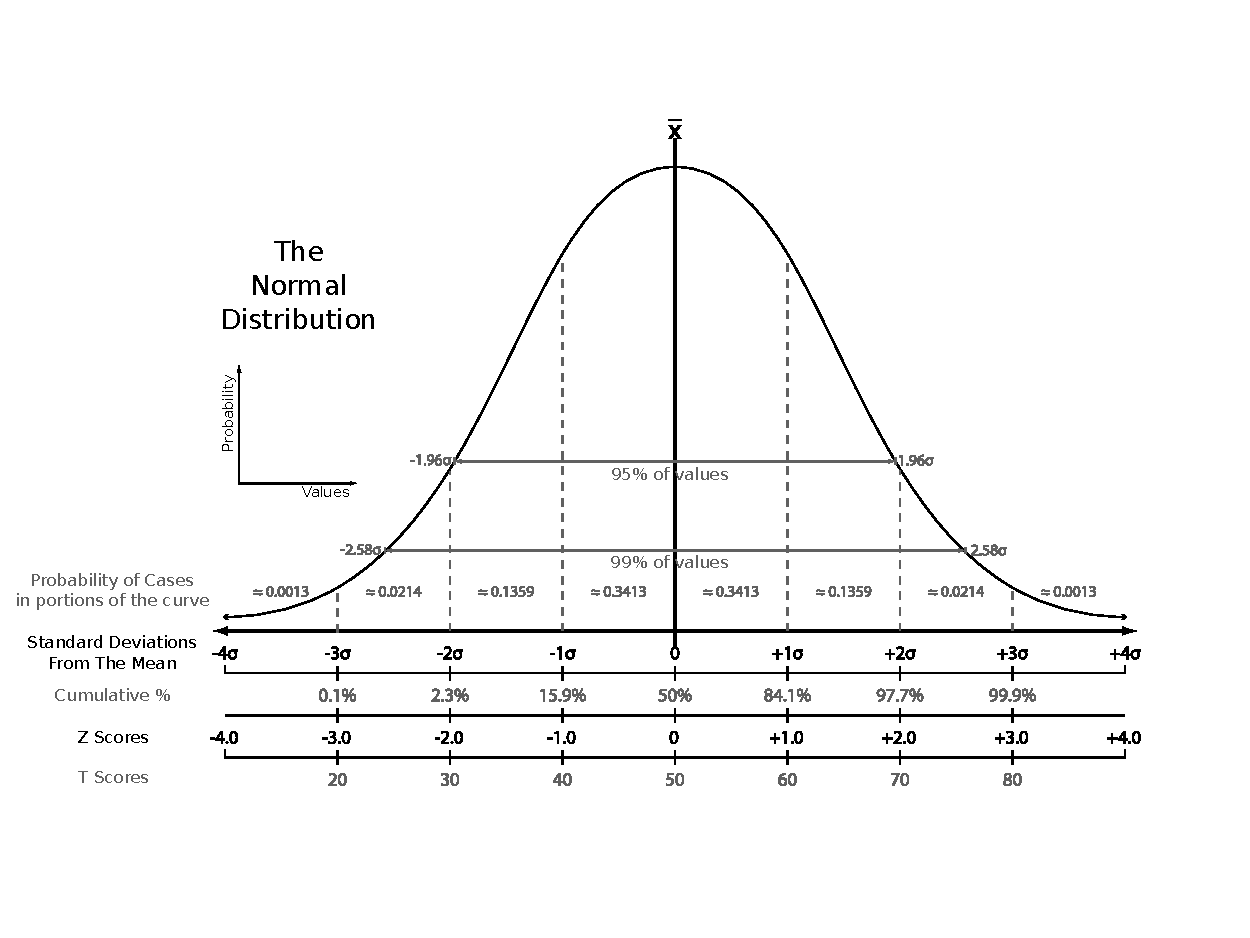
\includegraphics[width=0.8\textwidth]{The_Normal_Distribution.pdf}
	\caption{Визуализация понятия стандартизированного значения~(z-score) для~нормального распределения \cite{Wiki:z-score}}\label{fig:z-score}
\end{figure}
Среднее для~\textit{U} вычисляется по~формуле:
\begin{equation}\label{eq:U-mean}
m_{U} = \frac{n_{1}n_{2}}{2}.
\end{equation}
Формула стандартного отклонения в~случае отсутствия связок выглядит следующим образом:
\begin{equation}\label{eq:standard-deviation-no-ties}
\sigma_{U} =  \sqrt{\frac{n_{1}n_{2}(n_{1}+n_{2}+1)}{12}}.
\end{equation}
В~случае наличия связок используется другая формула:
\begin{equation}\label{eq:standard-deviation-ties}
\sigma_{U_{ties}} = \sqrt{\frac{n_{1}n_{2}(n_{1}+n_{2}+1)}{12} - \frac{n_{1}n_{2}\sum_{k=1}^{K}({t_{k}}^{3} - t_{k})}{12n(n-1)}} = \sqrt{\frac{n_{1}n_{2}}{12} \left((n+1)-\frac{\sum_{k=1}^{K}({t_{k}}^{3} - t_{k})}{n(n-1)}\right)},
\end{equation}
где~${\textstyle t_{k}}$ "--- количество наблюдений, имеющих ранг~\textit{k}, \textit{K} "--- общее число рангов, имеющих связки.
Далее, получив стандартизированное значение~(z-score), и~используя аппроксимацию стандартного нормального распределения, вычисляется \textit{p-значение} для~заданного уровня значимости (как~правило 0.05). Интерпретация результата осуществляется следующим образом:
\begin{equation}\label{eq:p-interpretation}
	\begin{aligned}
	p &\leq 0.05 \Rightarrow \text{нулевая гипотеза отклоняется}\\
	p &> 0.05 \Rightarrow \text{нулевая гипотеза не может быть отклонена}.
	\end{aligned}
\end{equation}
%
При~этом существует и~альтернативный вариант интерпретации:
%
\begin{equation}\label{eq:p-interpretation-2}
\begin{aligned}
p &< 0.05 \Rightarrow \text{нулевая гипотеза отклоняется}\\
p &\geq 0.05 \Rightarrow \text{нулевая гипотеза не может быть отклонена}.
\end{aligned}
\end{equation}
На~сегодняшний день нет~однозначной позиции, как~следует интерпретировать ситуацию, когда $p = \alpha$. В~данной работе используется вариант, описанный в~\ref{eq:p-interpretation}.

\section{Соотношение с~другими статистическими тестами}
\subsection{Сравнение U-теста Манна-Уитни-Уилкоксона c~t-тестом Стьюдента}
Часто можно услышать о~том, что~U-тест является непараметрическим аналогом t-теста, предназначенным для~данных, чьё~распределение отличается от~нормального. С~чисто практической точки зрения действительно можно сказать, что~в~случае нормального распределения определение наличия существенной разницы между двумя выборками целесообразно проводить посредством t-теста, в~случае отличия распределения от~нормального "--- U-теста. Таким образом, можно сказать, что~эти~тесты используются в~одной и~той~же цели.

При~этом, математический смысл U-теста и~t-теста существенно отличается. Как~уже было сказано ранее U-тест предназачен для~проверки нулевой гипотезы, заключающейся в~том, что~для~случайно выбранных из~двух выборок наблюдений ${\textstyle x \in X}$ и~${\textstyle y \in Y}$ вероятность того, что~\textit{x} больше \textit{y}, равна вероятности того, что~\textit{y} больше~\textit{x}, альтернативная гипотеза несёт утверждение о~том, что~эти~вероятности не~равны. В~то~же время t-тест предназначен для~проверки нулевой гипотезы о~равенстве средних двух~выборок, при~этом альтернативная гипотеза заключается в~том, что~средние двух выборок не~равны. В~связи с~этим, при~сравнении этих тестов следует иметь ввиду, что~в~общем случае, U-тест и~t-тест проверяют разные нулевые гипотезы, хотя и~имеющие отчасти схожий практический смысл. Результат U-теста чаще всего очень близок к~результату двухвыборочного t-теста для~ранжированных данных.
Далее в~таблице~\ref{tab:U-test-t-test-comparison} проводится общее сравнение U-теста с~t-тестом.
%
\begin{table}[ht]
	\caption{Свойства U-теста относительно t-теста}  \label{tab:U-test-t-test-comparison}
	\centering
	\begin{tabularx}{\textwidth}{p{0.25\linewidth} p{0.7\linewidth}} 
		\hline
		Свойство&Описание\\
		\hline
		Применимость к~порядковым данным&В~случае работы с~порядковыми~(ранговыми), а~не~количественными данными применение U-теста является предпочтительным относительно применения t-теста, при~этом следует помнить, что~расстояние между соседними значениями вариационного ряда нельзя считать постоянным.\\
		\hline
		Робастность&Поскольку U-тест работает с~суммой рангов, а~не~значений признаков, он~реже чем, t-тест ошибочно указывает на~значимость вследствие наличия выбросов. Однако, в~целом U-тест больше подвержен ошибке первого рода в~случае, когда данные одновременно обладают свойством гетероскедастичности и~имеют распределение отличное от~нормального.\\
		\hline
		Эффективность&В~случае нормального распределения асимптотическая эффективность U-теста составляет $\frac{3}{4}\pi \approx 0.95$ от~показателя t-теста~\cite{U-test-efficiency}. В~случае существенного отличия распределения от~нормального и~достаточно большого числа наблюдений эффективность U-теста существенно превышает эффективность t-теста~\cite{Practical-Nonparametric-Statistics}. Однако такое сравнение эффективности следует интерпретировать с~осторожностью, поскольку U-тест и~t-тест проверяют разные гипотезы и~оценивают разные величины. В~случае, например, потребности в~сравнении средних значений применение U-теста не~является оправданным в~принципе.\\
		\hline
	\end{tabularx}
\end{table}
%
\subsection{Альтернативные тесты в~случае неравенства распределений}
В~случае необходимости проверки стохастического упорядочивания двух выборок (т.\,е~альтернативной гипотезы $P(Y>X)+0.5P(Y=X)\neq0.5$) без~предположения о~равенстве их~распределений (т.\,е.~когда нулевая гипотеза имеет вид: $P(Y>X)+0.5P(Y=X)=0.5$, но~не~$F(X)=G(Y)$), следует использовать более подходящие тесты. К~ним~относятся, в~т.\,ч.~тесты Брунера-Мунцеля~\cite{Bruner-Munzel-test}, представляющий собой устойчивый к~гетероскедастичности аналог U-теста и~Флигнера-Поличелло~\cite{Fligner-Policello-test}, представляющий собой тест на~равенство медиан. В~частности, в~случае использовании более общей нулевой гипотезы $P(Y>X)+0.5P(Y=X)=0.5$ U-тест может достаточно часто приводить к~возникновению ошибки первого рода даже в~случае работы с~большими выборками (в~особенности в~случае неравенства дисперсий и~существенно различающегося объёма выборок), вследствие чего в~таких случаях использование альтернативных тестов будет предпочтительным~\cite{U-test-vs-Bruner-Munzel-test}. Таким образом, в~случае отсутствия предположения о~равенстве распределений в~случае справедливости нулевой гипотезы, использование альтернативных тестов будет являться предпочтительным.

В~случае проверки гипотезы сдвига при~существенно отличающихся распределениях U-тест может дать ошибочную интерпретацию значимости~\cite{U-test-unequal-variance}, вследствие чего в~таких условиях предпочтительным будет использование \href{https://en.wikipedia.org/wiki/Welch's_t-test}{варианта t-теста}~\cite{Welch-t-test}, предназначенного для~случаев неравных дисперсий~\cite{U-test-unequal-variance}.

В~ряде случаев может быть оправданным преобразование количественных данных в~ранги и~последующее проведение t-теста в~том~или~ином его~варианте в~зависимости от~предположений о~равенстве дисперсий. При~преобразовании количественных данных в~порядковые исходные дисперсии не~будут сохранены, их~следует пересчитать для~самих рангов. В~случае равенства дисперсий подходящей непараметрической заменой \href{https://en.wikipedia.org/wiki/F-test}{F-теста}~\cite{F-test} может являться тест \href{https://en.wikipedia.org/wiki/Brown-Forsythe_test}{Брауна-Форсайта}.
%
\subsection{Связь между U-тестом и~задачами классификации}\label{U-test&classification}
U-тест представляет собой частный случай \href{https://en.wikipedia.org/wiki/Ordered_logit}{модели упорядоченного выбора} (\foreignlanguage{english}{ordered logit model})~\cite{Ordered-logit}.
%
\section{Связь между U-тестом и~понятиями \foreignlanguage{english}{Receiver operating characteristic~(ROC), Area under curve~(AUC)}}\label{U-AUC}
Основываясь на~сказанном в~\ref{U-test&classification}, можно сделать вывод о~том, что~U-тест является не~только тестом для~проверки гипотезы сдвига~(либо иной аналогичной по~смыслу), но~и~представляет собой некий классификатор. Забегая вперёд можно сказать, что~смысл U-теста как~классификатора заключается в~следующем:
\begin{itemize}
	\item существует <<позитивный>> исход сравнения двух случайных наблюдений, заключающийся в~том, что~наблюдение из~$X$ больше наблюдения из~$Y$;
	\item проводится оценка доли суммы рангов <<позитивных>> элементов;
	\item как~и~в~целом c~ROC, в~случае, если значение доли <<позитивных>> элементов превышает 0.5, это~говорит о~том, что~классификатор в~целом выполняет свою функцию, в~случае равенства 0.5 "--- его~эффективность равнозначна угадыванию с~помощью подбрасывания монеты, в~случае значения менее 0.5 "--- использование такого классификатора даёт обратный результат.	 
\end{itemize}
На~первый взгляд, связь между U-тестом и~ROC не~выглядит очевидной. В~данной секции будет предпринята попытка разобраться в~том, почему эти~понятия всё~же имеют связь, и~в~чём заключается суть U-теста как~классификатора.

Сам~ROC-анализ не~входит в~периметр данного материала. Поэтому рассмотрим лишь его~основные моменты.
\begin{description}
	\item[ROC-кривая \foreignlanguage{english}{(ROC-curve: Receiver Operator Characteristic)} "---] график, позволяющий оценить качество бинарной классификации, отображает соотношение между долей объектов от~общего количества носителей признака, верно классифицированных как~несущие признак (\foreignlanguage{english}{true positive rate~(\emph{TPR})}, называемой \emph{чувствительностью алгоритма классификации}), и~долей объектов от~общего количества объектов, не~несущих признака, ошибочно классифицированных как~несущие признак (\foreignlanguage{english}{false positive rate~(\emph{FPR})}, величина \emph{1-FPR} называется \emph{специфичностью алгоритма классификации}) при~варьировании порога решающего правила. Также известна как~\textbf{кривая ошибок}. Анализ классификаций с применением ROC-кривых называется \textbf{ROC-анализом}. 
\end{description}
Количественная интерпретация ROC даёт показатель AUC~(\foreignlanguage{english}{Area Under Curve}, площадь под кривой). AUC "--- это~площадь, ограниченная ROC-кривой и~осью доли ложных положительных классификаций (ось абсцисс). Чем~выше показатель AUC, тем~качественнее классификатор, при~этом значение 0.5 демонстрирует непригодность выбранного метода классификации (соответствует случайному угадыванию с~помощью монеты). Значение менее 0.5 говорит, что~классификатор действует с~точностью до~наоборот: если положительные результаты назвать отрицательными и~наоборот, классификатор будет работать лучше~\cite{Wiki:ROC}.

Введём некоторые термины.
\begin{itemize}
	\item[P "---] количество объектов в~выборке, обладающих некоторым признаком (\foreignlanguage{english}{Condition positive}).
	\item[N "---] количество объектов в~выборке, не~обладающих некоторым признаком (\foreignlanguage{english}{Condition negative}).
	\item[TP "---] результат теста, корректно определивший наличие существующего в~действительности~(\foreignlanguage{english}{Positive}) признака (\foreignlanguage{english}{True positive}, истинно положительный).
	\item[TN "---] результат теста, корректно определивший отсутствие несуществующего в~действительности~(\foreignlanguage{english}{Negative}) признака (\foreignlanguage{english}{True negative}, истинно отрицательный).
	\item[FP "---] результата теста, ошибочно определивший наличие несуществующего в~действительности~(\foreignlanguage{english}{Negative}) признака (\foreignlanguage{english}{False positive}, ложно положительный).
	\item[FN "---] результат теста, ошибочно определивший отсутствие существующего в~действительности~(\foreignlanguage{english}{Positive}) признака (\foreignlanguage{english}{False negative}, ложно отрицательный).
\end{itemize}
На~основании вышесказанного можно создать таблицу~\ref{tab:ROC-contingency-table} сопряжённости результатов применения бинарного классификатора. Строки содержат данные о~фактическом наличии либо отсутствии признака, столбцы "--- предсказанном~(\foreignlanguage{english}{predicted}) с~помощью классификатора.
%
\begin{table}[ht]
	\caption{Таблица сопряжённости результатов работы бинарного классификатора}  \label{tab:ROC-contingency-table}
	\centering
	\begin{tabularx}{\textwidth}{p{0.2\linewidth} p{0.375\linewidth} p{0.375\linewidth}} 
		\hline
		Всего $P+N$&Predicted Positive~(PP)&Predicted negative~(PN)\\
		\hline
		Positive~(P)&TP&FN, ошибка второго рода~\cite{Wiki:type-1-2-errors}\\
		\hline
		Negative~(N)&FP, ошибка первого рода~\cite{Wiki:type-1-2-errors}&TN\\
		\hline
	\end{tabularx}
\end{table}
%
Как~видно из~таблицы~\ref{tab:ROC-rates} бинарный классификатор может приводить к~возникновению ошибок двух типов. Введём ещё~несколько определений и~определим формулы для~расчёта вероятностей исходов его~работы.
\begin{table}[ht]
	\caption{Возможные исходы применения бинарного классификатора}\label{tab:ROC-rates}
	\centering
	\begin{tabularx}{\textwidth}{p{0.15\linewidth} p{0.4\linewidth} p{0.4\linewidth}} 
		\hline
		Показатель&Формула&Альтернативные названия\\
		\hline
	    TPR~(SEN)&\begin{equation}\label{TPR}
	    TPR=\frac{TP}{P}=1-FNR
	    \end{equation}&\foreignlanguage{english}{True positive rate, Recall, Sensitivity, Probability of~detection, hit rate, power}, чувствительность\\
		\hline
	    FPR&\begin{equation}\label{FPR}
	    FPR = \frac{FP}{N} = 1 - TNR
	    \end{equation}&\foreignlanguage{english}{False positive rate, probability of~false alarm, fall-alarm}\\
		\hline
		FNR&\begin{equation}\label{FNR}
		FNR = \frac{FN}{P} = 1 - TPR
		\end{equation}&False negative rate, miss rate\\
		\hline
		TNR~(SPC)&\begin{equation}\label{TNR}
		TNR = \frac{TN}{N} = 1 - FPR
		\end{equation}&\foreignlanguage{english}{True negative rate, specifitity, selectivity}, специфичность\\
		\hline
	\end{tabularx}
\end{table}
%
Вероятность TPR может быть записана как:
\begin{equation}\label{eq:TPR-probability}
P_{TPR} = \mathbb{P}(1|x\in C_{1}),
\end{equation}
что~означает, что~если объект~$x$ принадлежит классу~$C_{1}$, то~данный показатель 
...
\clearpage

\chapter{Практическая реализация}\label{U-test-practice}
\section{Реализация в~табличном процессоре LibreOffice Calc}\label{U-test-spreadsheet}
На~данный момент можно c~уверенностью сказать, что~табличные процессоры являются стандартом для~расчётов оценщиков. Проникновение средств разработки в~профессиональную деятельность, например языков программирования Python и~R,  идёт достаточно медленно. Кроме того, самостоятельный поэтапный расчёт позволяет лучше понять методику U-теста. Поэтому было принято решение создать пошаговую инструкцию для~проведения U-теста в~электронной таблице. Для~этого был использован программный продукт LibreOffice Calc~(Version: 7.3.3.2, Ubuntu package version: 1:7.3.3~rc2-0ubuntu0.20.04.1~lo1 Calc: threaded), существенная часть функционала которого имеется также и~в~наиболее распространённом приложении такого рода "--- \foreignlanguage{english}{Microsoft Excel}. Отсутствуют основания полагать, что~сделанные расчёты не~будут корректно работать в~приложениях, отличных от~LibreOffice Calc. Однако гарантировать это~также невозможно. Для~однозначно корректного проведения теста рекомендуется использовать именно данное приложение, имеющее версии для~всех основных операционных систем. Актуальная версия файла~\href{https://github.com/Kirill-Murashev/AI_for_valuers_book/blob/main/Parts-Chapters/Mann-Whitney-Wilcoxon/U-test.ods}{U-test.ods} находится в~\href{https://github.com/Kirill-Murashev/AI_for_valuers_book/tree/main/Parts&Chapters/Mann-Whitney-Wilcoxon}{репозитории} вместе с~остальными материалами данной работы.

Данные, рассматриваемые в~данной подсекции, являются вымышленными и~были созданы алгоритмом генерации псевдослучайных чисел LibreOffice Calc. Для~повторной генерации необходимо использовать сочетание клавиш \emph{ctrl+shift+F9}. 

Рассмотрим учебную задачу. В~ячейках I3:J30 содержатся данные значений некоторого количественного признака для~двух выборок, взятых из~множеств \textit{I} и~\textit{J} соответственно. Различие между элементами этих множеств заключается в~наличии некоторого признака у~элементов множества \textit{I} и~его~отсутствии у~элементов множества \textit{J}. Задача заключается в~проверке гипотезы о~том, что~различие в~данном признаке следует признать существенным, а~сам признак является ценообразующим фактором. Выдвинем нулевую гипотезу, сформулировав её~в~трёх вариантах, соответствующих трём уровням строгости, описанным ранее в~таблице~\ref{tab:nul-hypothesis-variants}. Следует отметить, что~U-тест входит в~периметр т.\,н.~\emph{частотного подхода к~вероятности} (о~различиях между \emph{частотным} и~\emph{байесовским} подходами к~вероятности применительно к~оценке стоимости можно прочитать, в~частности в~\cite{Murashev:freq-baye-prob}). Как~известно, частотный подход базируется на~предпосылке о~том, что случайность является следствием объективной неопределённости, которая может быть уменьшена только путём проведения серии экспериментов. В частотном подходе существует чёткое разделение на~случайные и~неслучайные параметры. Типичной задачей является оценка тех~или~иных параметров генеральной совокупности, представляющей собой набор случайных величин, на~основе детерминированных параметров выборки, например: среднее, мода, дисперсия и~т.\,д. Последние представляют собой конкретные значения, в~которых уже~нет~никакой случайности. Таким образом, принимая фундаментальное предположение о~случайном характере изучаемых величин, мы~применяем те~или~иные методы математической статистики, позволяющие получить конкретные значения оценок параметров. Из~этого следует, что~нулевая гипотеза чаще всего <<пессимистична>>, т.\,е.~несёт утверждение, что~в~основе исследуемого явления или~процесса лежит случайность, вследствие чего мы~не~имеем возможность делать надёжные выводы. С~учётом всего вышесказанного, сформулируем нулевую и~альтернативную гипотезы~(таблица~\ref{tab:nul-alt-hypothesis-variants}) в~трёх вариантах, согласно уровням строгости, показанным в~таблице~\ref{tab:nul-hypothesis-variants}.
\begin{table}[ht]
	\caption{Нулевая и~альтернативная гипотезы при~анализе тестовых данных}  \label{tab:nul-alt-hypothesis-variants}
	\centering
	\begin{tabularx}{\textwidth}{p{0.15\linewidth} p{0.4\linewidth} p{0.4\linewidth}} 
		\hline
		Тип гипотезы&Нулевая гипотеза (H0)&Альтернативная гипотеза (H1)\\
		\hline
		Научная&Распределение удельных показателей стоимости одинаково для~объектов-аналогов, обладающих признаком <<X>> (множество объектов \textit{I}), и~не~обладающих им (множество объектов \textit{J}), сдвиг между ними отсутствует, статистические оценки, сделанные для~одного множества объектов-аналогов, являются несмещёнными для~другого.&Распределение удельных показателей стоимости для~объектов из~множества~I отличается от~распределения, имеющего место у~множества~J, существует сдвиг, оценка, сделанная для~объектов, принадлежащих одному множеству, будет смещённой для~объектов, принадлежащих другому.\\
		\hline
		Практическая&Медианное значение удельного показателя стоимости объектов, обладающих признаком~<<X>>, не~отличается от~медианного значения удельного показателя стоимости объектов, не~обладающих признаком~<<X>>, "--- их~медианы равны.&Медианное значение удельного показателя стоимости объектов, обладающих признаком~<<X>>, отличается от~медианного значения удельного показателя стоимости объектов, не~обладающих признаком~<<X>>, "--- их~медианы не~равны.\\
		\hline
		Изложенная в~терминах оценки&Наличие или~отсутствие признака~<<X>> не~оказывает сколько-нибудь заметного влияния на~стоимость "--- признак <<X>> не~является ценообразующим фактором.&Наличие или~отсутствие признака~<<X>> оказывает влияние на~стоимость "--- признак <<X>> является ценообразующим фактором.\\ \hline
	\end{tabularx}
\end{table}
Ячейки C2:C19 содержат некоторые описательные статистики.  Для~удобства первичного анализа бывает полезно показать свойства выборок графически. На~рисунке~\ref{fig:BoxPlot} изображена диаграмма <<ящик с~усами>>~(\foreignlanguage{english}{Boxplot}), позволяющая сделать некоторые выводы на~основе одного взгляда. Как~видно, значения средних и~медиан двух выборок различны. При~этом также отличаются минимальные значения. При~этом максимальное значение одинаково. Также следует обратить внимание, что~несмотря на~то, что~среднее и~медиана первой выборки превышают аналогичные показатели второй, минимальное значение первой меньше чем~у~второй. В~таких условиях ещё~сложнее сделать вывод о~том, является~ли различие в~признаке существенным, или~же разница в~показателе стоимости носит случайный характер.
%
\begin{figure}[ht]
	\centering
	\includegraphics[width=0.95\textwidth]{BoxPlot.pdf}
	\caption{Диаграмма <<ящик с~усами>> (Boxplot) для~обеих выборок }
	\label{fig:BoxPlot}
\end{figure}
%
Следующим подготовительным этапом является проверка нормальности распределения значений количественного признака (в~данном случае условного показателя удельной стоимости). Существует ряд строгих тестов, позволяющих провести такую проверку численными методами. В~подсекциях~\ref{U-test-Python} и~\ref{U-test-R} будут показаны соответствующие способы проведения такого теста. В~данном разделе ограничимся графическим способом. На~рисунках~\ref{fig:s1-hist}, \ref{fig:s2-hist} изображены гистограммы распределения частот для~первой и~второй выборок соответственно, совмещённые с~кривыми функции плотности вероятности для~нормального распределения.
%
\begin{figure}[ht]
	\centering
	\includegraphics[width=0.95\textwidth]{s1-hist.pdf}
	\caption{Гистограмма первой выборки, совмещённая с~кривой функции плотности вероятности для~нормального распределения}
	\label{fig:s1-hist}
\end{figure}
%
\begin{figure}[ht]
	\centering
	\includegraphics[width=0.95\textwidth]{s2-hist.pdf}
	\caption{Гистограмма второй выборки, совмещённая с~кривой функции плотности вероятности для~нормального распределения}
	\label{fig:s2-hist}
\end{figure}
%

Как~видно на~диаграммах, форма распределения обеих выборок существенно отличается от~формы кривой функции плотности вероятности нормального распределения. При~работе с~реальными данными в~любом случае необходимо проводить количественные тесты проверки на~нормальность распределений, однако на~данном этапе остановимся на~интерпретации диаграмм и~сделаем вывод о~том, что~распределения обеих выборок отличаются от~нормального, что~позволяет сделать вывод о~неприменимости параметрических методов статистического оценивания и~необходимости использования непараметрических, к~числу которых относится и~U-тест.

При~работе с~электронной таблицей отсутствует потребность в~отдельном построении общего вариационного ряда для~двух выборок. Вместо этого можно сразу перейти к~вычислению рангов наблюдений. С~учётом возможного наличия связок (повторяющихся значений) следует использовать функцию \texttt{RANK.AVG}, последовательно указав при~этом три~аргумента: наблюдение, для~которого вычисляется ранг, диапазон всех значений общего вариационного ряда, тип сортировки: 0 "--- по~убыванию, 1 "--- по~возрастанию, в~нашем случае необходимо указать~1. Столбцы L, N содержат дублирующие значения, столбцы M и~O "--- ранги соответствующих наблюдений. 

После этого проведём подсчёт сумм рангов для~каждой из~выборок в~ячейках~C20:C21. В~ячейке~C22 проведём подсчёт общей суммы рангов обеих выборок. Для~проверки рассчитаем тот~же показатель согласно формуле~\ref{eq:common-R}.

Далее в~ячейках C25, C26 по~формулам~\ref{eq:U1}, \ref{eq:U2} вычислим соответственно значения ${\textstyle U_1,\ U_{2}}$. После чего проверим корректность контрольного соотношения~\ref{eq:check-U-value} в~ячейке D27. В~C28 выбираем меньшее значение, которое и~будет использоваться в~дальнейшем в~качестве U-статистики. В~нашем случае меньшее значения U-статистики у~выборки из~множества~\textit{J}.

Рассчитаем показатель CLES. Для~этого используем формулу~\ref{eq:CLES}. Результат содержится в~C29. В~рассматриваемом примере значение показателя составляет 0.39477, что~следует интерпретировать следующим образом: <<вероятность того, что~значение показателя удельной стоимости случайно выбранного наблюдения из~множества~$J$ превышает аналогичный показатель случайно выбранного наблюдения из~множества~$I$ составляет 0.39477~(39.48\,\%)>>.

Далее рассчитаем значение коэффициента рангово-бисериальной корреляции по~формулам~\ref{eq:RBC-formula-1}, \ref{eq:RBC-formula-2}, разместив его~в~ячейке~C36. В~рассматриваемом случае значение составило 0.21, что~говорит о~том, что~сила корреляционной связи между наличием у~объекта признака <<X>> и~удельным показателем его~стоимости составляет~0.21.

После этого перейдём к~расчёту стандартизированного значения согласно формуле~\ref{eq:z-score}. Для~этого в~ячейке C37 рассчитаем среднее по~формуле~\ref{eq:U-mean}, а~затем перейдём к~вопросу расчёта стандартного отклонения. Следует отметить, что~для~этого существуют две формулы: одна~(\ref{eq:standard-deviation-no-ties}) применяется в~случае отсутствия связок (ячейка C38), вторая~(\ref{eq:standard-deviation-ties}) "--- при~их~наличии (ячейка C39). В~рассматриваемом случае связки имели место. Их~обработка осуществлялась в~столбцах P и~Q, а~также в~ячейках E35:E49. В~результате было получено два значения, отличие между которыми составило менее одного процента. Учёт фактора связок необходим с~точки зрения максимальной научной корректности результата, однако в~повседневной практической деятельности некоторые оценщики могут столкнуться со~сложностями с~корректным учётом фактора связок, а~также не~иметь достаточно времени для~дополнительных расчётов. Практический опыт говорит о~том, что~сколько-нибудь существенное отличие значений стандартного отклонения, полученных с~помощью формулы~\ref{eq:standard-deviation-ties} от~значений, полученных согласно~\ref{eq:standard-deviation-no-ties}, бывает в~случаях большого числа связок, а~также наличия крупных групп. В~остальных ситуациях более простая формула, автоматически вычисляющая показатель~${\textstyle \sigma}$, даёт корректный результат, достаточный для~практического применения в~оценке. В~любом случае, решение об~использовании строгих либо простых методов принимает сам~оценщик. В~рассматриваемом примере учёт фактора связок был осуществлён. 

Зная среднее арифметическое и~стандартное отклонение, вычисляем z-метку в~ячейке C44 (поскольку одной из~предпосылок U-теста является непрерывность распределения, а~эмпирические данные имеют дискретное, при~вычислении z-метки используется поправка), а затем, используя аппроксимацию стандартного нормального распределения, "--- p-значение. В~рассматриваемом примере оно~составило~0.173. Используя правило~\ref{eq:p-interpretation}, приходим к~выводу о~невозможности отклонить нулевую гипотезу. Таким образом, используя формулировку, наиболее близкую к~оценочной деятельности (см.~таблицу~\ref{tab:nul-alt-hypothesis-variants}), можно придти к~следующему выводу: наличие или~отсутствие признака~<<X>> не~оказывает сколько-нибудь заметного влияния на~стоимость "--- признак <<X>> не~является ценообразующим фактором.

Для~лучшей интерпретации результата построим ROC кривую~(диаграмма~\ref{fig:ROC-curve-spreadsheet}). Графические средства табличного процессора сильно уступают возможностям средств разработки, поэтому качество диаграммы оставляет желать лучшего, однако она~всё~же даёт возможность сделать некоторые интересные выводы. Следует отметить, что~построение ROC кривой и~её~дальнейшая интерпретация носят лишь приблизительный характер и~дают точность приближения в~пределах нескольких процентов. Для~точного анализа следует использовать профессиональные средства разработки, в~частности описанные в~подсекциях~\cref{U-test-Python,U-test-R}.
%
\begin{figure}[ht]
	\centering
	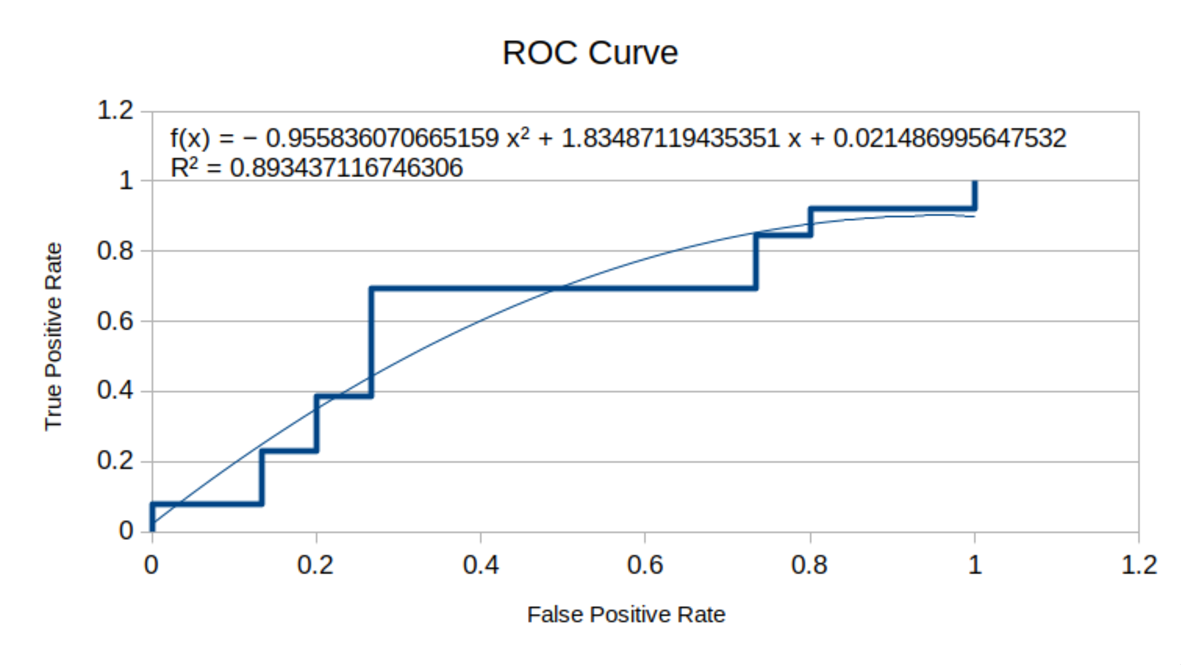
\includegraphics[width=0.95\textwidth]{ROC-curve-spreadsheet.pdf}
	\caption{ROC кривая для~тестовых данных}
	\label{fig:ROC-curve-spreadsheet}
\end{figure}
% 

LibreOffice Calc не~имеет штатных средств расчёта площади под~кривой. Поэтому используем её~аппроксимацию полиномом второй степени, получив в~результате следующее выражение:
\begin{equation*}\label{eq:ROC-curve-spreadsheet-polynom-approx-1}
f(x)=-0.955836070665159x^2 + 1.83487119435351x+0.021486995647532,
\end{equation*}
округляемое до
\begin{equation*}\label{eq:ROC-curve-spreadsheet-polynom-approx-2}
f(x)=-0.95584x^2 + 1.83487x+0.02149.
\end{equation*}
Для~нахождения площади под~аппроксимирующей кривой решим определённый интеграл вида
\begin{equation*}\label{eq:AUC-integral-0}
\int_{0}^{1}(-0.95584x^2 + 1.83487x+0.02149)~dx.
\end{equation*}
Преобразуем выражение в~более удобное:
\begin{equation*}\label{eq:AUC-integral-1}
\int_{0}^{1}(-\frac{2987x^2}{3125} + \frac{183487x}{100000}+ \frac{2149}{100000})~dx.
\end{equation*}
Далее вычислим значение определённого интеграла.
\begin{equation*}\label{eq:AUC-integral-2}
\begin{aligned}
&\text{Проинтегрируем выражение почленно и~выделим константу:}\\
&-\frac{2987}{3125} \int_{0}^{1} x^{2}~dx + \frac{183487x}{100000} \int_{0}^{1}x~dx + \frac{2149}{100000} \times \int_{0}^{1} 1~dx.\\
&\text{Известно, что~первообразной функции}\ x^2\ \text{является}\ \frac{x^3}{3}, \\
&\text{тогда} \left(-\frac{2987x^{3}}{9375}\right)_{0}^{1} + \frac{183487x}{100000} \int_{0}^{1}x~dx + \frac{2149}{100000} \times \int_{0}^{1} 1~dx.\\
&\text{Рассчитаем антипроизводные первого члена в~пределах и~вычислим разность:}\\ &\left(-\frac{2987x^{3}}{9375}\right)_{0}^{1} = \left(-\frac{2987 \times 1^{3}}{9375}\right) - \left(-\frac{2987 \times 0^{3}}{9375}\right) = -\frac{2897}{9375},\\
&\text{подставив затем в~общее выражение:} -\frac{2897}{9375} + \frac{183487x}{100000} \int_{0}^{1}x~dx + \frac{2149}{100000} \times \int_{0}^{1} 1~dx.\\
& \text{Таже известно, что~первообразной функции}\ x\ \text{является}\ \frac{x^2}{2}, \\
&\text{тогда}\ -\frac{2897}{9375} + \left(\frac{183487x}{100000}\right)_{0}^{1} + \frac{2149}{100000} \times \int_{0}^{1} 1~dx.\\
&\text{Рассчитаем антипроизводные второго члена в~пределах и~вычислим разность:}\\
&\left(\frac{183487x}{100000}\right)_{0}^{1} = \left(\frac{183487 \times 1^2}{100000}\right) - \left(\frac{183487 \times 0^2}{100000}\right) = \left(\frac{183487x}{100000}\right),\\
&\text{подставив затем в~общее выражение:} \frac{359293}{600000} + \frac{2149}{100000} \times \int_{0}^{1} 1~dx.\\
&\text{Известно, что~первообразной 1 является x,}\\
&\text{тогда}\ \frac{359293}{600000} + \left(\frac{2149}{100000}\right)_{0}^{1}\\
&\text{Рассчитаем антипроизводные третьего члена в~пределах и~вычислим разность:}\\
&\left(\frac{2149}{100000}\right)_{0}^{1} = \frac{2149 \times 1}{100000} - \frac{2149 \times 0}{100000} = \frac{2149}{100000},\\
&\text{подставив затем в~общее выражение:}\ \frac{372187}{600000}=0.621312
\end{aligned}
\end{equation*}
Полученное значение приблизительно соответствует значению показателя CLES, по~мере увеличения степени аппроксимирующего полинома абсолютная разница между значениями AUC и~CLES будет уменьшаться, стремясь к~нулю при~приближении степени полинома к~$\dfrac{N}{2}-1$.

В~данной подсекции мы~рассмотрели пошаговый расчёт статистики критерия, а~также осуществили интерпретацию результата. Следует отметить, что, несмотря на~возможность и~даже относительное удобство такого варианта проведения U-теста, предпочтение всё~же следует отдавать профессиональным средствам разработки в~области машинного обучения и~статистического вывода, например, языкам программирования Python или~R, о~которых и~пойдёт речь ниже.
%

\clearpage

\section{Реализация на~Python}\label{U-test-Python}
%
\lstset{language=Python,
	basicstyle=\ttfamily,
	keywordstyle=\color{Blue}\ttfamily,
	stringstyle=\color{Red}\ttfamily,
	commentstyle=\color{Emerald}\ttfamily,
	morecomment=[l][\color{Magenta}]{\#},
	breaklines=true,
	breakindent=0pt,
	breakatwhitespace,
	columns=fullflexible,
	showstringspaces=false
}
%
В~сфере машинного обучения и, в~особенности, в~ряде областей таких как~\foreignlanguage{english}{deep learning} язык Python уже~стал де~факто стандартом. Кроме того, он~универсален и~прекрасно подходит для~разработки тех~или~иных экспертных систем. Его~популярность означает в~т.\,ч.~наличие огромного количества обучающих материалов по~всем аспектам разработки в~области анализа данных, предназначенных для~пользователей любого уровня подготовки. При~этом, большая часть необходимых оценщику вычислений можно провести путём вызова готовых функций из~подключаемых библиотек, предназначенных для~анализа данных, без~необходимости написания большого объёма кода и~без~глубоких знаний в~области программирования. По~мнению автора данной работы, будущее оценки заключается именно в~применении экспертных систем, основанных на~обучении моделей на~основе наборов данных открытых рынков. Как~будет показано ниже, применение Python существенно сокращает время проведения U-теста, а~также позволяет создавать визуализации исследуемого рынка, не~прибегая к~сторонним средствам. Кроме того, использование готовых функций практически исключает вероятность возникновения ошибок в~расчётах. При~написании кода была использована версия языка Python 3.9.12, а~также IDE Spyder (5.1.5). Код в~формате скрипта доступен по~\href{https://github.com/Kirill-Murashev/AI_for_valuers_book/blob/main/Parts-Chapters/Mann-Whitney-Wilcoxon/U-test.py}{ссылке}~\cite{Murashev:U-test.py}, код в~формате \foreignlanguage{english}{Python Notebook}  доступен по~\href{https://github.com/Kirill-Murashev/AI_for_valuers_book/blob/main/Parts-Chapters/Mann-Whitney-Wilcoxon/U-test.ipynb}{ссылке}~\cite{Murashev:U-test.ipynb}.

Рассмотрим реальный набор данных, содержащий сведения об~удельных показателях стоимости квартир в~Санкт-Петербургской агломерации. Данные были собраны 28~сентября~2021~года с~сайта \href{https://www.cian.ru/}{cian.ru} и~доступны по~\href{https://github.com/Kirill-Murashev/datasets/blob/main/Saint-Petersburg/flats/spba_flats_210928.csv}{ссылке}~\cite{ds:spba-flats-210928}. Рассматриваемый набор данных содержит 34821~наблюдение. Как~известно, Санкт-Петербургская агломерация включает в~себя как~территории, входящие в~состав города федерального значения, так~и~те, которые формально относятся к~Ленинградской области. При~этом, разделение на~город и~область носит чисто юридический характер. С~социально-экономической точки зрения, ближайшие территории Ленинградской области неразрывно связаны с~Санкт-Петербургом и~являются частью одной агломерации, к~слову, крупнейшей в~мире на~такой широте. При~формировании запросов, использованных в~процессе скрепинга, южная граница агломерации была установлена примерно по~оси автодороги А-120, северная "--- автодороги 41А-189. При~этом в~её состав были включены некоторые населённые пункты за~пределами этих границ, например, города Кировск и~Шлиссельбург.

Сформулируем задачу. Необходимо установить наличие либо отсутствие статистически значимого различия в~ценах объектов, расположенных в~границах самого Санкт-Петербурга, и~объектов, формально расположенных в~Ленинградской области. Аналогично предыдущему случаю, сформулируем нулевую и~альтернативную гипотезы, имеющие на~этот раз практический смысл (см.~таблицу~\ref{tab:nul-alt-hypothesis-SPba}).
\begin{table}[ht]
	\caption{Нулевая и~альтернативная гипотезы при~анализе данных Санкт-Петербургской городской агломерации}  \label{tab:nul-alt-hypothesis-SPba}
	\centering
	\begin{tabularx}{\textwidth}{p{0.15\linewidth} p{0.4\linewidth} p{0.4\linewidth}} 
		\hline
		Тип гипотезы&Нулевая гипотеза (H0)&Альтернативная гипотеза (H1)\\
		\hline
		Научная&Распределение удельных показателей стоимости квартир, расположенных в~границах Санкт-Петербурга, и~квартир, расположенных на~прилегающих к~нему территориях Ленинградской области, одинаково, сдвиг между ними отсутствует, статистические оценки, сделанные для~множества объектов-аналогов, расположенных в~одной части агломерации, являются несмещёнными для~объектов, расположенных в~другой.&Распределение удельных показателей стоимости квартир, расположенных в~границах Санкт-Петербурга отличается от~распределения удельных показателей стоимости квартир, расположенных на~прилегающих к~нему территориях Ленинградской области, существует сдвиг, оценка, сделанная для~объектов, расположенных в~одной части агломерации, будет смещённой для~объектов, расположенных в~другой её~части.\\
		\hline
		Практическая&Медиана удельного показателя стоимости квартир, расположенных в~границах Санкт-Петербурга, равна медиане удельного показателя стоимости квартир, расположенных на~прилегающих территориях Ленинградской области.&Медиана удельного показателя стоимости квартир, расположенных в~границах Санкт-Петербурга не~равна медиане удельного показателя стоимости квартир, расположенных на~прилегающих территориях Ленинградской области.\\
		\hline
		Изложенная в~терминах оценки&Расположение квартиры в~границах Санкт-Петербурга либо на~прилегающих к~нему территориях Ленинградской области не~является существенным различием и~не~требует какого-либо специального учёта.&Расположение квартиры в~границах Санкт-Петербурга либо на~прилегающих к~нему территориях Ленинградской области является существенным различием и~требует отдельный учёт.\\ \hline
	\end{tabularx}
\end{table}

Язык \foreignlanguage{english}{Python} изначально не~был создан специально для~анализа данных. Поэтому в~его базовой версии могут отсутствовать многие функции, необходимые для~проведения расчётов. К~счастью, для~решения задач в~области машинного обучения и~анализа данных существует ряд подключаемых библиотек, содержащих множество необходимых функций. Их~количество и~широта решаемых задач не~столь велики как, например, у~языка~R, однако они~являются исчерпывающими для~более чем~95\,\% задач, стоящих перед оценщиками. Для~решения задач, рассматриваемых в~данном материале, потребуются следующие библиотеки: \foreignlanguage{english}{numpy, pandas, math, matplotlib.pyplot, scipy.stats}. Для~их~подключения используем код, представленный в~скрипте~\ref{lst:import-libraries-Python}.
\begin{lstlisting}[float, caption = Подключение необходимых библиотек, firstnumber=1, label= lst:import-libraries-Python]
# import libraries
import numpy as np
import pandas as pd
import math
import matplotlib.pyplot as plt
import scipy.stats as stats
from scipy.stats import norm
from scipy.stats import normaltest
from scipy.stats import shapiro
from scipy.stats import anderson
from scipy.stats import mannwhitneyu
\end{lstlisting}
%

Установим уровень значимости~${\textstyle \alpha}$, принимаемый для~всей дальнейшей работы. Выбор его~значения остаётся за~исследователем, однако в~работах по~эконометрике и~исследованию операций чаще всего встречается значение~\textit{0.05}, которое и~будет использовано. Для~задания значения уровня значимости используется код~\ref{lst:set-alpha}.
%
\begin{lstlisting}[float, caption = Задание применяемого уровня значимости, firstnumber=1, label= lst:set-alpha]
# set significance level
alpha = 0.05
\end{lstlisting}
% 

После~этого всё~готово для~начала работы. Создадим датафрейм на~основе текстового файла, содержащего изучаемый набор данных~(скрипт~\ref{lst:import-data-create-dataframe}).
%
\begin{lstlisting}[float, caption = Загрузка данных и~создание датафрейма, firstnumber=1, label= lst:import-data-create-dataframe]
# import dataset
df = pd.read_csv('spba-flats-210928.csv')
print(df)
type(df['price_m'])
\end{lstlisting}
%
Датафрейм в~точности повторяет содержимое исходного файла и~содержит 34821~наблюдения и~4~переменные: порядковый номер, ссылку на~объявление, показатель стоимости 1~кв.\,м, а~также код местоположения, состоящий из~четырёх букв: первая из~которых означает регион (s "--- Санкт-Петербург, l "--- Ленинградская область), вторая и~третья "--- административный район, три последних "--- муниципальное образование либо территорию. При~этом \foreignlanguage{english}{Python} добавил собственную переменную, содержащую номера наблюдений. Следует обратить внимание на~то, что~нумерация в~\foreignlanguage{english}{Python}, как~и~в~большинстве языков программирования, начинается не~с~единицы, а~с~нуля. Поскольку переменные, содержащие номера наблюдений и~ссылки на~объявления из~исходного файла, не~будут использоваться в~дальнейшем, создадим новый датафрейм, содержащий только необходимые переменные, а~также выгрузим из~виртуальной памяти первый датафрейм для~оптимизации ресурсов компьютера (листинг~\ref{lst:create-new-dataframe-release-RAM}). В~рассматриваемом случае такая микрооптимизация не~играет большой роли, однако в~целях выработки навыков написания хорошего кода, лучше всё~же написать одну дополнительную строку.
%
\begin{lstlisting}[float, caption = Создание датафрейма\, содержащего только необходимые переменные\, и~выгрузка из~памяти неиспользуемых данных, firstnumber=1, label= lst:create-new-dataframe-release-RAM]
# get only prices and counties, release RAM
df1 = df[['price_m', 'county']]
del [[df]]
\end{lstlisting}
%

Теперь в~распоряжении оценщика в~удобном виде есть рабочий датафрейм, содержащий данные о~рынке квартир всей агломерации Санкт-Петербурга. Для~формирования первого представления о~распределении построим гистограмму, совмещённую с~кривой плотности для~нормального распределения. Для~определения рационального числа интервалов (столбцов гистограммы)~$k$ используем формулу Heinhold-Gaede~cite\cite{Ingenieur-Statistik}:
\begin{equation}\label{eq:k-hist-Heinhold-Gaede}
k = \sqrt{n},
\end{equation}
где~\textit{n} "--- число наблюдений. Для~построения гистограммы используем скрипт~\ref{lst:price-hist-spba}.
%
\begin{lstlisting}[float, caption = Построение гистограммы для~агломерации Санкт-Петербурга, firstnumber=1, label= lst:price-hist-spba]
# calculate the number of observations on data frame
spbaLenR = round(math.sqrt(len(df1.index)))

# fit a normal distribution to the data: mean and standard deviation
mu, std = norm.fit(df1["price_m"])

# plot the histogram
plt.hist(df1["price_m"], bins=spbaLenR, density=True)

# plot the PDF
xmin, xmax = plt.xlim()
x = np.linspace(xmin, xmax, 100)
p = norm.pdf(x, mu, std)

plt.plot(x, p, 'k', linewidth=2)
title = "Fit Values: {:.2f} and {:.2f}".format(mu, std)
plt.title(title)

# save to .pdf
plt.savefig('spba-price-histogram-py.pdf')
\end{lstlisting}
%

Рассмотрим полученную гистограмму~\ref{fig:spba-prices-hist}. Ось~x содержит значения цен за~1\,кв.\,м, ось~y "--- значения вероятностей интервалов. Обе оси представлены в~стандартном виде. Также показаны значения матожидания и~стандартного отклонения для~теоретического нормального распределения. Как~видно, распределение имеет тяжёлый правый хвост, что~позволяет сделать предварительный вывод о~том, что~оно~отличается от~нормального. В~дальнейшем будет проведён строгий тест на~нормальность, пока~же можно ограничиться первичной субъективной интерпретацией гистограммы.
%
\begin{figure}[ht]
	\centering
	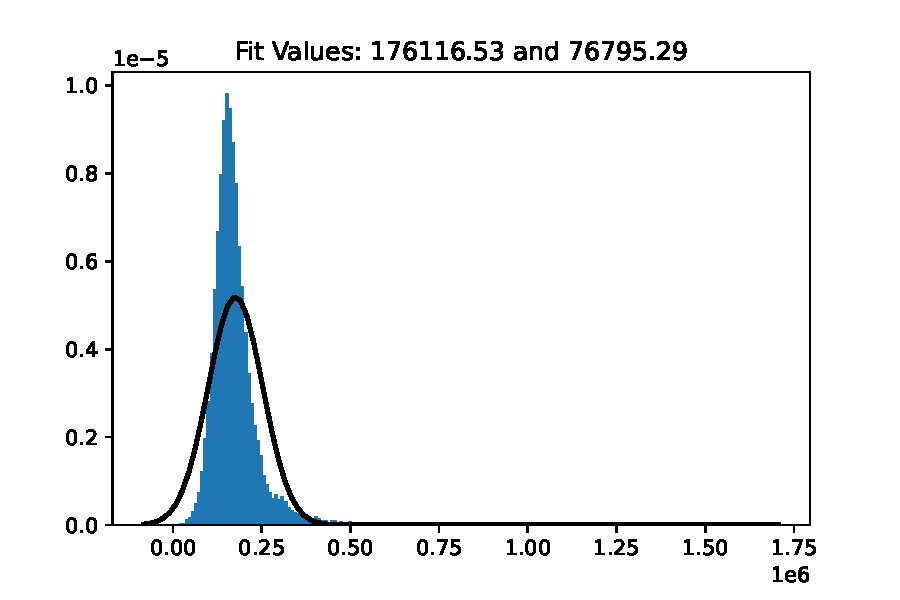
\includegraphics[width=0.95\textwidth]{spba-price-histogram-py.pdf}
	\caption{Гистограмма плотности распределения цен за~1\,кв.\,м квартир в~Санкт-Петербургской агломерации, совмещённая с~кривой функции плотности вероятности для~нормального распределения}
	\label{fig:spba-prices-hist}
\end{figure}
%
Поскольку предметом исследования является различие между объектами, расположенными в~двух частях агломерации, а~исходный набор данных содержит сведения о~наблюдениях из~обеих, потребуется создание двух отдельных датафреймов. Здесь следует сделать небольшое отступление: практический опыт говорит о~том, что~сам~анализ данных и~построение моделей занимают только 20\,\% времени, тогда как~80\,\% уходит на~сбор и~предобработку данных. Одним из~важных элементов этих процессов является правильная разметка данных. В~случае с~рассматриваемым набором данных их~анализ в~разрезе отдельных территорий вплоть до~уровня муниципалитетов был предусмотрен изначально путём указания индекса территории для~каждого наблюдения. Как~было сказано выше, первая буква индекса содержит указание на~то, в~какой части агломерации расположено наблюдение. В~этом случае, для~создания двух раздельных датафреймов достаточно двух строк, содержащих несложные регулярные выражения.
%
\begin{lstlisting}[float, caption = Создание отдельных датафреймов для~Санкт-Петербурга и~Ленинградской области, firstnumber=1, label= lst:create-two-separate-df-for-S-Pb-LO]
# create separate dataframes for city and suburbs
dfs = df1[df1['county'].str.startswith('s')] # Saint-Petersburg
dfl = df1[df1['county'].str.startswith('l')] # Leningradskaja oblastq
\end{lstlisting}
%
Датафрейм \emph{dfs} содержит данные для~наблюдений из~Санкт-Петербурга (28643 наблюдения), \emph{dfl} "--- Ленинградской области (6178 наблюдений). Построим гистограммы для~обеих частей агломерации (скрипты~\ref{lst:price-hist-spb}, \ref{lst:price-hist-lo}).
%
\begin{lstlisting}[float, caption = Построение гистограммы для~Санкт-Петербурга, firstnumber=1, label= lst:price-hist-spb]
# Saint-Petersburg
# calculate the number of observations on data frame
spbLenR = round(math.sqrt(len(dfs.index)))

# fit a normal distribution to the data: mean and standard deviation
muS, stdS = norm.fit(dfs["price_m"])

# plot the histogram
plt.hist(dfs["price_m"], bins=spbLenR, density=True)

# plot the PDF
xmin, xmax = plt.xlim()
x = np.linspace(xmin, xmax, 100)
ps = norm.pdf(x, muS, stdS)

plt.plot(x, ps, 'k', linewidth=2)
title = "S-Pb. Fit Values: {:.2f} and {:.2f}".format(muS, stdS)
plt.title(title)

# save to .pdf
plt.savefig('spb-price-histogram-py.pdf')
\end{lstlisting}
%
\begin{lstlisting}[float, caption = Построение гистограммы для~Ленингадской области, firstnumber=1, label= lst:price-hist-lo]
# LO
# calculate the number of observations on data frame
loLenR = round(math.sqrt(len(dfl.index)))

# fit a normal distribution to the data: mean and standard deviation
muL, stdL = norm.fit(dfl["price_m"])

# plot the histogram
plt.hist(dfl["price_m"], bins=loLenR, density=True)

# plot the PDF
xmin, xmax = plt.xlim()
x = np.linspace(xmin, xmax, 100)
pl = norm.pdf(x, muL, stdL)

plt.plot(x, pl, 'k', linewidth=2)
title = "LO. Fit Values: {:.2f} and {:.2f}".format(muL, stdL)
plt.title(title)

# save to .pdf
plt.savefig('lo-price-histogram-py.pdf')
\end{lstlisting} 
%
\begin{figure}[ht]
	\centering
	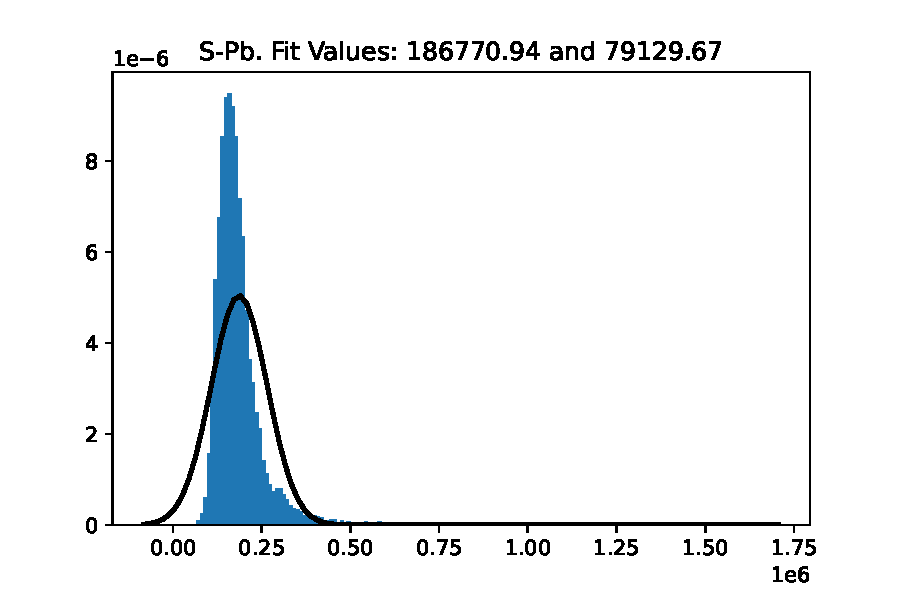
\includegraphics[width=0.95\textwidth]{spb-price-histogram-py.pdf}
	\caption{Гистограмма плотности распределения цен за~1\,кв.\,м квартир в~Санкт-Петербурге, совмещённая с~кривой функции плотности вероятности для~нормального распределения}
	\label{fig:spb-prices-hist}
\end{figure}
%
\begin{figure}[ht]
	\centering
	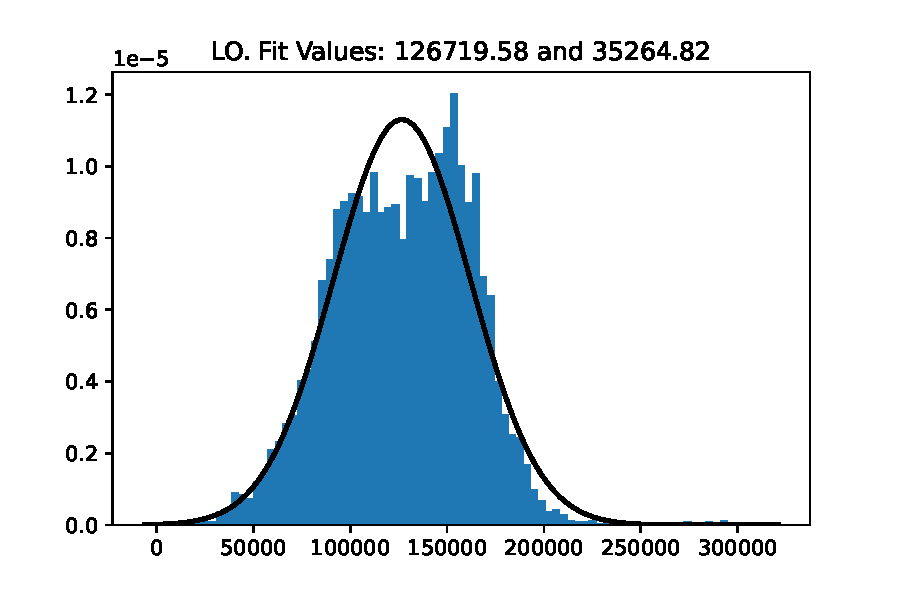
\includegraphics[width=0.95\textwidth]{lo-price-histogram-py.pdf}
	\caption{Гистограмма плотности распределения цен за~1\,кв.\,м квартир в~Ленинградской области, расположенных в~границах агломерации Санкт-Петербурга, совмещённая с~кривой функции плотности вероятности для~нормального распределения}
	\label{fig:lo-prices-hist}
\end{figure}
%

Гистограмму иногда путают со~столбчатой диаграммой. Следует напомнить, что~правильно построенная гистограмма является отображением вероятностных свойств данных, сумма площадей всех её~прямоугольников равна единице, а~по~оси~$y$ отложены значения вероятностей диапазонов (столбцов гистограммы), а~не~число наблюдений в~каждом диапазоне. Как~видно из~гистограммы~\ref{fig:spb-prices-hist}, распределение удельных цен в~Санкт-Петербурге, также как~и~в~случае с~распределением цен для~всей агломерации, имеет тяжёлый правый хвост. При~этом распределение цен для~объектов агломерации, находящихся за~пределами границ Санкт-Петербурга, показанное на~гистограмме~\ref{fig:lo-prices-hist} выглядит относительно симметрично.

Также построим график <<ящик с~усами>> для~обоих датафреймов с~помощью скрипта~\ref{lst:boxplot-spba} (см.~диаграмму~\ref{fig:spb-lo-boxplot-py}). Как~видно, значение медианы цен объектов, расположенных в~Санкт-Петербурге, выше значения третьего квартиля цен объектов, расположенных на~прилегающих территориях Ленинградской области.
%
\begin{lstlisting}[float, caption = Построение диаграммы <<ящик с~усами>>~(boxplot) для~обеих подвыборок, firstnumber=1, label= lst:boxplot-spba]
# add labels to data
dfs["region"] = "SPb"
dfl["region"] = "LO"

# plot boxplot
prices = [dfs, dfl]
allPrices = pd.concat(prices)
plt.figure()
allPrices.boxplot(by="region")

# save to .pdf
plt.savefig('spb-lo-boxplot-py.pdf')
\end{lstlisting} 
%
\begin{figure}[ht]
	\centering
	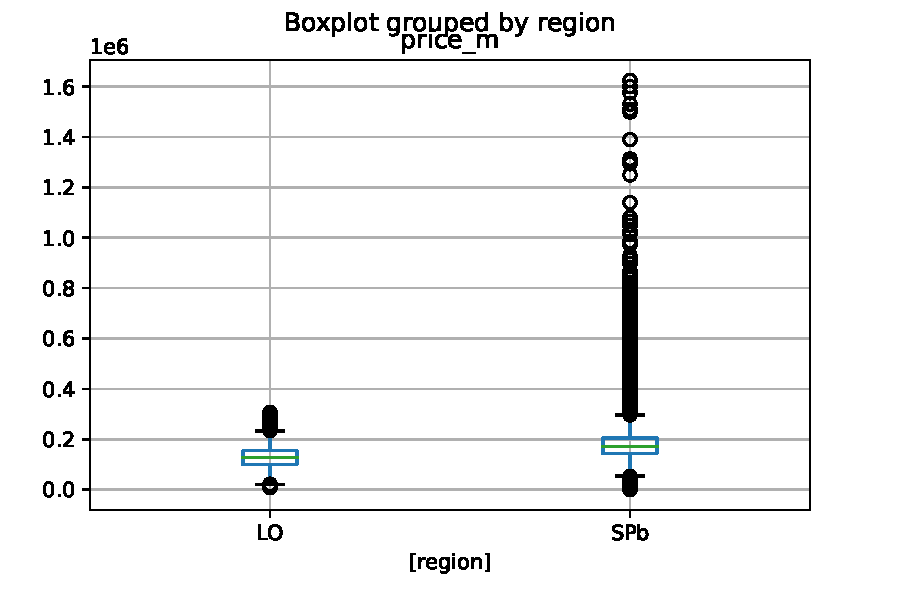
\includegraphics[width=0.95\textwidth]{spb-lo-boxplot-py.pdf}
	\caption{Диаграмма <<ящик с~усами>> для~цен предложений квартир в~Санкт-Петербургской агломерации в~разрезе региональной принадлежности}
	\label{fig:spb-lo-boxplot-py}
\end{figure}
%

Данные обстоятельства позволяет сделать субъективное предположение о~том, что~нулевую гипотезу следует отклонить. Однако графические методы анализа подходят только для~быстрой первичной интерпретации, а~также для~презентационных целей. Для~формирования объективного доказательного суждения потребуется проведение самого U-теста. 

Для~проверки применимости U-теста следует провести тест на~нормальность распределения для~обоих датафреймов (\textit{dfs}, \textit{dfl}). Существует множество критериев для~проверки гипотезы о~нормальности распределения выборки. В~данном случае были использованы три~теста:
\begin{itemize}
	\item тест Шапиро"--~Франчиа~\cite{Shapiro-Wilk-test};
	\item тест ${\textstyle K^{2}}$ Д'Агостино~\cite{Agostino-test};
	\item тест Андерсона"--~Дарлинга~\cite{Anderson-Darling-test}.
\end{itemize}
Тест Шапиро"--~Франчиа оценивает выборку данных и~вычисляет, насколько вероятно, что~она~была взята из~генеральной совокупности, имеющей нормальное распределение. Данный тест считается одним из~наиболее мощных тестов проверки на~нормальность~\cite{Kobzarq-prikl-mathstat}. При~этом существуют некоторые предпосылки, указывающие на~то, что~он хорошо работает на~выборках среднего размера, не~превышающих пяти тысяч наблюдений (минимальное количество должно быть не~менее пяти). 

Тест ${\textstyle K^{2}}$ Д'Агостино основывается на~анализе показателей \href{https://en.wikipedia.org/wiki/Skewness}{асимметрии}~\cite{Wiki:skewness} и~\href{https://en.wikipedia.org/wiki/Kurtosis}{эксцесса}~\cite{Wiki:kurtosis}, представляющих собой третий и~четвёртый \href{https://en.wikipedia.org/wiki/Central_moment}{центральные моменты}~\cite{Wiki:central-moment} соответственно. Данный тест также считается одним из~наиболее мощных и~не~имеет ограничений по~максимальному числу наблюдений.

Тест Андерсона"--~Дарлинга представляет собой модифицированную версию \href{Wiki:Kolmogorow-Smirnow-test}{критерия согласия Колмогорова"--~Смирнова}~\cite{Wiki:Kolmogorow-Smirnow-test} и~используется для~проверки гипотезы о~том, что~эмпирическое распределения согласуется с~одним из~известных теоретических. В~отличие от~двух предыдущих тестов, его~результатом является не~p-значение, а~статистика критерия, что~требует более сложной интерпретации результата, которая однако легко автоматизируется.

Сформулируем нулевые гипотезы:
\begin{itemize}
	\item H0(SPb): распределение значений удельных цен предложений квартир в~Санкт-Петербурге не~отличается от~нормального;
	\item H0(LO): распределение значений удельных цен предложений квартир на~территориях Ленинградской области, входящих в~агломерацию Санкт-Петербурга, не~отличается от~нормального.
\end{itemize}
Таким образом всего будет выполнено 6~тестов, результаты которых сведены в~таблицу~\ref{tab:normality-tests-values}. В~отношении данных по~Санкт-Петербургу все~три теста позволили отклонить \emph{H0(SPb)}, два~из трёх тестов также позволили отклонить \emph{H0(LO)}. На~основании данных результатов можно сделать вывод о~том, что~распределение одной из~выборок однозначно отличается от~нормального, второй "--- отличается от~нормального с~высокой вероятностью. В~связи с~этим, применение параметрических тестов для~сравнения двух выборок является неуместным, вследствие чего следует использовать рассмотренный выше U-тест.
\begin{lstlisting}[float, caption = Тест Шапиро-Уилка для~данных по~Санкт-Петербургу, firstnumber=1, label= lst:shapiro-wilk-test-spb]
stat, p = shapiro(dfs['price_m'])
print('Statistics=%.3f, p=%.3f' % (stat, p))
# interpret
if p <= alpha:
print('Sample does not look Gaussian (reject H0)')
else:
print('Sample looks Gaussian (fail to reject H0)')
\end{lstlisting}
%
\begin{lstlisting}[float, caption = Тест Шапиро-Уилка для~данных по~Ленинградской области, firstnumber=1, label= lst:shapiro-wilk-test-lo]
stat, p = shapiro(dfl['price_m'])
print('Statistics=%.3f, p=%.3f' % (stat, p))
# interpret
if p <= alpha:
print('Sample does not look Gaussian (reject H0)')
else:
print('Sample looks Gaussian (fail to reject H0)')
\end{lstlisting}  
%
\begin{lstlisting}[float, caption = Тест K2 Агостино для~данных по~Санкт-Петербургу, firstnumber=1, label= lst:K^2-D'Agostino-test-spb]
stat, p = normaltest(dfs['price_m'])
print('Statistics=%.3f, p=%.3f' % (stat, p))
# interpret
if p <= alpha:
print('Sample does not look Gaussian (reject H0)')
else:
print('Sample looks Gaussian (fail to reject H0)')
\end{lstlisting}
%
\begin{lstlisting}[float, caption = Тест K2 Агостино для~данных по~Ленинградской области, firstnumber=1, label= lst:K^2-D'Agostino-test-lo]
stat, p = normaltest(dfl['price_m'])
print('Statistics=%.3f, p=%.3f' % (stat, p))
# interpret
if p <= alpha:
print('Sample does not look Gaussian (reject H0)')
else:
print('Sample looks Gaussian (fail to reject H0)')
\end{lstlisting}  
%
\begin{lstlisting}[float, caption = Тест Андерсона-Дарлинга для~данных по~Санкт-Петербургу, firstnumber=1, label= lst:Anderon-Darling-test-spb]
result = anderson(dfs['price_m'])
print('Statistic: %.3f' % result.statistic)
p = 0
for i in range(len(result.critical_values)):
sl, cv = result.significance_level[i], result.critical_values[i]
if result.statistic < result.critical_values[i]:
print('%.3f: %.3f, data looks normal (fail to reject H0)' % (sl, cv))
else:
print('%.3f: %.3f, data does not look normal (reject H0)' % (sl, cv))
\end{lstlisting}
%
\begin{lstlisting}[float, caption = Тест Андерсона-Дарлинга для~данных по~Ленинградской области, firstnumber=1, label= lst:Anderon-Darling-test-lo]
result = anderson(dfl['price_m'])
print('Statistic: %.3f' % result.statistic)
p = 0
for i in range(len(result.critical_values)):
sl, cv = result.significance_level[i], result.critical_values[i]
if result.statistic < result.critical_values[i]:
print('%.3f: %.3f, data looks normal (fail to reject H0)' % (sl, cv))
else:
print('%.3f: %.3f, data does not look normal (reject H0)' % (sl, cv))
\end{lstlisting}  
%
\begin{table}[ht]
	\caption{Результаты проведения тестов проверки данных по~Санкт-Петербургской агломерации на~нормальность $({\textstyle \alpha=0.05})$}\label{tab:normality-tests-values}
	\centering
	\begin{tabular}{lll}
		\hline
		Тест&Санкт-Петербург&Ленинградская область\\
		\hline
		Шапиро"--~Уилка:&\ref{lst:shapiro-wilk-test-spb}&\ref{lst:shapiro-wilk-test-lo}\\
		статистика критерия~(W)&0.689&0.991\\
		p-значение&0.000&0.000\\
		H0&отклоняется&отклоняется\\
		\hline
		${\textstyle K^{2}}$ Д'Агостино:&\ref{lst:K^2-D'Agostino-test-spb}&\ref{lst:K^2-D'Agostino-test-lo}\\
		статистика критерия~(${\textstyle K^{2}}$)&28166.251&4.067\\
		p-значение&0.000&0.131\\
		HO&отклоняется&не~может быть отклонена\\
		\hline
		Андерсона"--~Дарлинга:&\ref{lst:Anderon-Darling-test-spb}&\ref{lst:Anderon-Darling-test-lo}\\
		статистика критерия~(${\textstyle A^{2}}$)&1688.671&15.795\\
		H0:&отклоняется&отклоняется\\
		\hline
		Итоговый вывод:&&\\
		H0&отклоняется&отклоняется\\
		\hline
	\end{tabular}
\end{table}
Теперь остаётся только провести сам~U-тест. Для~этого используем скрипт~\ref{lst:u-test-spba}. Его~результаты представлены в~таблице~\ref{tab:u-test-py-result}. Поскольку p-значение меньше заданного уровня значимости, можно сделать практический вывод о~том, что~различия в~показателях стоимости объектов, расположенных в~границах Санкт-Петербурга, и~объектов, расположенных на~территориях его~агломерации, расположенных в~Ленинградской области, являются существенными и~требуют соответствующий учёт. Другие интерпретации результата могут быть получены из~столбца <<Альтернативная гипотеза~(H1)>> таблицы~\ref{tab:nul-alt-hypothesis-SPba}.
%
\begin{lstlisting}[float, caption = Проведение теста Манна"--~Уитни-Уилкоксона для~данных удельных цен предложения квартир в~агломерации Санкт-Петербурга, firstnumber=1, label= lst:u-test-spba]
stat, p = mannwhitneyu(dfs['price_m'], dfl['price_m'])
print('stat=%.3f, p=%.3f' % (stat, p))
if p <= 0.05:
print('Probably different distributions')
else:
print('Probably the same distribution')
\end{lstlisting}  
%
\begin{table}[ht]
	\caption{Результаты проведения U-теста для~данных Санкт-Петербургской агломерации $({\textstyle \alpha=0.05})$}\label{tab:u-test-py-result}
	\centering
	\begin{tabular}{ll}
		\hline
	Показатель&Значение\\
		\hline
	Статистика критерия&142555441.000\\
		\hline
	p-значение&0.000\\
		\hline
	Нулевая гипотеза (см.~таблицу~\ref{tab:nul-alt-hypothesis-SPba})&отклоняется\\
		\hline
	\end{tabular}
\end{table}

\clearpage

\section{Реализация на~R}\label{U-test-R}
%
\lstset{language=R,
	basicstyle=\ttfamily,
	keywordstyle=\color{Blue}\ttfamily,
	stringstyle=\color{Red}\ttfamily,
	commentstyle=\color{Emerald}\ttfamily,
	morecomment=[l][\color{Magenta}]{\#},
	breaklines=true,
	breakindent=0pt,
	breakatwhitespace,
	columns=fullflexible,
	showstringspaces=false
}
%
Язык программирования~R не~столь распространён как~Python, хотя и~пользуется достаточной популярностью в~развитых странах. В~Северной Евразии область его~применения является достаточно нишевой и, чаще всего, он~используется в~научной деятельности, в~особенности в~области биологии и~химии. Для~специалиста по~машинному обучению знание данного языка является скорее бонусом, но~не~основным навыком. Тем~не~менее, следует отметить достоинства~R, к~которым можно отнести:
\begin{itemize}
	\item большой набор библиотек и~функций, существенно превосходящий набор средств Python;
	\item очень хорошие средства визуализации результата;
	\item удобные инструменты разработки веб-приложений, например Shiny;
	\item язык является не~компилируемым, а~интерпретируемым, что~зачастую удобнее в~случае решения конкретных задач.
\end{itemize}
Последнее обстоятельство является, пожалуй, главным аргументом в~пользу включения языка~R в~цикл публикаций по~искусственному интеллекту для~оценщиков. Если Python как~язык общего назначения изначально предназначен для~создания компилируемых исполняемых приложений, R разработан для~пошагового анализа данных и~представления всех промежуточных результатов. 

Выбор основного языка программирования, используемого оценщиком, зависит от~конкретной задачи: в~случае разработки крупных комплексных решений предпочтительнее использование Python. В~ситуациях, когда целью является решение частной задачи, в~особенности требующей серьёзной визуализации результата, есть смысл обратить внимание на~R. В~любом случае оба~этих языка обладают достаточным набором средств для~решения всего спектра задач по~анализу данных, возникающих в~процессе оценки стоимости.

При~написании кода на~R была использована его~версия 4.2.0 (2022-04-22) \foreignlanguage{english}{--- "Vigorous Calisthenics"}, а~также \foreignlanguage{english}{IDE RStudio (RStudio 2022.02.2+485 "Prairie Trillium" Release (8acbd38b0d4ca3c86c570cf4112a8180c48cc6fb, 2022-04-19) for Ubuntu Bionic)}. 

Рассмотрим ещё~одну практическую задачу на~примере набора данных о~рынке жилья города Алматы, предоставленный профессором университета <<Нархоз>> G.\,Shoulenbaeva. Файл с~данными доступен по~\href{https://github.com/Kirill-Murashev/AI_for_valuers_book/blob/main/Parts-Chapters/Mann-Whitney-Wilcoxon/almaty-apts-2019-1.csv}{ссылке}\cite{ds:almaty-apts-2019-1}. Рассматриваемый набор данных содержит 2355 наблюдений, а~также 12~переменных, содержащих сведения о~значениях признаков наблюдений. Одна из~переменных содержит сведения о~том, предлагается~ли квартира к~продаже вместе с~мебелью и~бытовой техникой или~без~них. Возможны три~варианта значения переменной:
\begin{itemize}
	\item продажа квартиры без~мебели и~техники;
	\item продажа квартиры с~частичным оснащением предметами интерьера и~техники;
	\item продажа полностью оснащённой квартиры. 
\end{itemize}
Сформулируем задачу: необходимо установить наличие либо отсутствие влияния оснащения квартиры предметами движимого имущества на~её~стоимость. Данная задача, по~мнению автора, представляет определённый теоретический и~практический интерес. Во-первых, теория оценки гласит, что~при~определении стоимости объекта недвижимости следует учитывать стоимость только неотделимых улучшений объекта, тогда как~стоимость элементов, являющихся движимым имуществом, следует исключать из~стоимости самого объекта. При~этом, на~практике зачастую невозможно точно определить принадлежность того или~иного элемента к~отделимым либо неотделимым улучшениям, а~также определить их~наличие у~объектов-аналогов. Математический анализ данных рынка позволит ответить на~вопрос, существует~ли данная проблема в~принципе, либо влияние фактора наличия улучшений, имеющих признаки отделимых, слишком несущественно и~в~любом случае не~может быть корректно учтено при~проведении оценки. Во~вторых, решение данной задачи даст новые знания о~конкретном рынке недвижимого имущества. Для~дальнейшего анализа будем считать, что~существуют только два~варианта:
\begin{itemize}
	\item продажа без~потенциально отделимых улучшений и~движимого имущества;
	\item продажа вместе с~потенциально отделимыми улучшениями и~движимым имуществом.
\end{itemize}
Решение объединить две категории в~одну продиктовано, во-первых, математическими ограничениями U-теста, предназначенного для~сравнения только двух выборок (для~анализа более чем~двух выборок существует непараметрический тест \href{https://en.wikipedia.org/wiki/Kruskal–Wallis_one-way_analysis_of_variance}{Краскела--~Уоллиса} также известный как~односторонний ранговый ANOVA~\cite{Wiki:Kruskal-Wallis}), во-вторых, с~точки зрения обозначенной выше теоретической проблемы, важно понять, оказывает~ли влияние на~стоимость факт наличия каких-либо отделимых улучшений как~таковых, в~третьих, деление объектов на~частично и~полностью оснащённые могло носить несколько субъективный характер. Варианты нулевой и~альтернативной гипотез приведены в~таблице~\ref{tab:nul-alt-hypothesis-almaty}.
\begin{table}[ht]
	\caption{Нулевая и~альтернативная гипотезы при~анализе данных Алматы}  \label{tab:nul-alt-hypothesis-almaty}
	\centering
	\begin{tabularx}{\textwidth}{p{0.15\linewidth} p{0.4\linewidth} p{0.4\linewidth}} 
		\hline
		Тип гипотезы&Нулевая гипотеза (H0)&Альтернативная гипотеза (H1)\\
		\hline
		Научная&Распределения удельных показателей стоимости квартир, предлагаемых к~продаже вместе с~отделимыми улучшениями и~движимым имуществом, и~квартир, продаваемых без~них, одинаковы, сдвиг между ними отсутствует, статистические оценки, сделанные для~множества объектов-аналогов, продаваемых вместо с~отделимыми улучшениями и~движимым имуществом, являются несмещёнными для~объектов, продаваемых без~них (справедливо и~обратное утверждение).&Распределение удельных показателей стоимости квартир, предлагаемых к~продаже вместе с~отделимыми улучшениями и~движимым имуществом, и~квартир, продаваемых без~них, различается, существует сдвиг, оценка, сделанная для~объектов, предлагаемых к~продаже вместе с~отделимыми улучшениями и~движимым имуществом, будет смещённой для~объектов, предлагаемых к~продаже без~них (справедливо и~обратное утверждение).\\
		\hline
		Практическая&Медиана удельного показателя стоимости квартир, предлагаемых к~продаже вместе с~отделимыми улучшениями и~движимым имуществом, равна медиане удельного показателя стоимости квартир, предлагаемых к~продаже без~них&Медиана удельного показателя стоимости квартир, предлагаемых к~продаже вместе с~отделимыми улучшениями и~движимым имуществом, не~равна медиане удельного показателя стоимости квартир, предлагаемых к~продаже без~них.\\
		\hline
		Изложенная в~терминах оценки&Наличие либо отсутствие отделимых улучшений и~движимого имущества в~составе продаваемой квартиры не~является существенным различием и~не~требует какой-либо специальный учёт, т.\,е.~не~является ценообразующим фактором.&Наличие либо отсутствие отделимых улучшений и~движимого имущества в~составе продаваемой квартиры является существенным различием и~требует специальный учёт, т.\,е.~является ценообразующим фактором.\\
		\hline
	\end{tabularx}
\end{table}

При~написании кода на~R автор использовал его~версию~4.2.0, а~также \foreignlanguage{english}{IDE RStudio (version 2022.02.2 Build 485)}. При~начале работы следует подключить необходимые библиотеки, задать некоторые константы, а~также установить адрес рабочего каталога, например так, как~это показано в~скрипте~\ref{lst:import-libraries-set-constants-set-catalog-R}.
%
\begin{lstlisting}[float, caption = Подключение библиотек и~задание значений констант и~адреса рабочего каталога, firstnumber=1, label= lst:import-libraries-set-constants-set-catalog-R]
# activate libraries
library(tidyverse)
library(moments)
library(ggplot2)
library(gamlss)
library(normtest)
library(nortest)

# set constants
options('scipen'=2, 'digits'=3)
set.seed(19190709)

# set work catalog
setwd('~/.../Mann-Whitney-Wilcoxon/')
\end{lstlisting}  
%

Далее необходимо создать датафрейм на~основе существующего текстового файла с~данными. Затем в~целях оптимизации использования ресурсов желательно оставить только необходимые переменные 'price.m' и~'furniture', а~затем преобразовать датафрейм~в~более удобный и~современный формат 'tibble' (скрипт~\ref{lst:create-dataframe-transform-and-convert-R}). После этого необходимо рассчитать общее число наблюдений, а~также каждого типа в~зависимости от~наличия отделимых улучшений (скрипт~\ref{lst:calculate-numbers-of-observations-R}). Результаты подсчёта представлены в~таблице~\ref{tab:numbers-of-observations-almaty-R}.
%
\begin{lstlisting}[float, caption = Создание датафрейма и его настройка, firstnumber=1, label= lst:create-dataframe-transform-and-convert-R]
# create data set from file, create subset with needed variables,
# change the type of object to a more convenient and modern one
almatyFlats <- read.csv('almaty-apts-2019-1.csv', header = TRUE, sep = ",", dec = ".")
myvars <- c('price.m', 'furniture')
almatyFlats <- almatyFlats[myvars]
as_tibble(almatyFlats)
\end{lstlisting} 
%
\begin{lstlisting}[float, caption = Подсчёт количества наблюдений, firstnumber=1, label= lst:calculate-numbers-of-observations-R]
# calculation of the total number of observations,
# as well as depending on the equipment 
n.total <- nrow(almatyFlats)
n.non.equip <- NROW(almatyFlats$furniture[ which(almatyFlats$furniture == 0)])
n.equip <- NROW(almatyFlats$furniture[ which(almatyFlats$furniture > 0)]))
\end{lstlisting}
%

В~целях первичной визуализации данных построим гистограммы для~всех наблюдений. Число столбцов на~этот раз будет определено по~формуле, разработанной в~1991 году P.\,W.~Nowiczkij~\cite{Nowiczkij:oczenka-pogresh}:
\begin{equation}\label{eq:k-hist_Nowiczkij}
k = \frac{1}{3}\sqrt[5]{\varepsilon^4 n^2} \equiv \frac{1}{3} \sqrt[5]{\frac{n^2}{\xi^8}}, 
\end{equation}
где~$\varepsilon$ "--- коэффициент эксцесса, $\xi$ "--- коэффициент контрэксцесса. Для~удобства, сначала создадим соответствующую функцию (скрипт~\ref{lst:k-number-Nowiczkij-R}). а~затем рассчитаем рациональное число интервалов для~всего набора данных~(скрипт~\ref{lst:k-number-R}), а~затем отдельно для~квартир, предлагаемых к~продаже без~отделимых улучшений и~с~ними. Результаты расчёта приведены в~таблице~\ref{tab:numbers-of-observations-almaty-R}.
%
\begin{lstlisting}[float, caption = Создание функции для~расчёта~k по~формуле P.\,W.~Nowiczkij, firstnumber=1, label= lst:k-number-Nowiczkij-R]
# create function for second Nowiczkij formula
kHistNowiczkij2 <- function(x, na.omit = FALSE){ # create function, ignore missed values
n   <- NROW(x)                                 # calculate n
kurt = kurtosis(x)                             # calculate kurtosis
kn2 = (((kurt^4)*(n^2))^(1/5))*(1/3)           # calculate k
return(kn2)                                    # return k  
}                                              # end of function
\end{lstlisting} 
%
\begin{lstlisting}[float, caption = Расчёт~k по~формуле P.\,W.~Nowiczkij для~наблюдений различных типов, firstnumber=1, label= lst:k-number-R]
# calculation numbers of k for different types of observations
k.all.data <- kHistNowiczkij2(almatyFlats$price.m)
k.non.equip <- kHistNowiczkij2(almatyFlats$price.m[ which(almatyFlats$furniture == 0)])
k.equip <-kHistNowiczkij2(almatyFlats$price.m[ which(almatyFlats$furniture > 0)])                                       
\end{lstlisting}
%
\begin{table}[ht]
	\caption{Сведения о~количестве наблюдений различных типов на~рынке города Алматы}\label{tab:numbers-of-observations-almaty-R}
	\centering
	\begin{tabular}{lll}
		\hline
		Тип наблюдений&Количество&Рациональное число интервалов~(k)\\
		\hline
		Все~наблюдения&2355&36\\
		\hline
		Наблюдения без~отделимых улучшений&605&22\\
		\hline
		Наблюдения с~отделимыми улучшениями&1750&31\\
		\hline
	\end{tabular}
\end{table}
%

Построим гистограммы для~всех наблюдений~(диаграмма ~\ref{fig:almaty-hist-all-r}), тех, которые имеют оснащение~\ref{fig:almaty-hist-equiped-r}, и~тех, которые продаются без~каких-либо отделимых улучшений~\ref{fig:almaty-hist-nequiped-r}. Из~диаграмм следует, что~распределения имеют тяжёлые правые хвосты, что~косвенно указывает на~то, что~распределение во~всех случаях отличается от~нормального. Для~обоснованного суждения в~дальнейшем будут выполнены количественные тесты проверки нормальности. Код для~построения гистограмм приведён в~скрипте~\ref{lst:plot-hist-R}. В~таблице~\ref{tab:summaries-almaty-R} содержатся базовые описательные статистики для~каждого из~трёх типов наблюдений, построенные при~помощи кода~\ref{lst:summaries-R}. Для~лучшего восприятия с~помощью скрипта~также была построена диаграмма <<ящик с~усами>>~(\foreignlanguage{english}{boxplot}) (скрипт~\ref{lst:boxplot-R}), приведённая на~рисунке~\ref{fig:almaty-boxplot-r}. Как~видно, медиана цен объектов, предлагаемых к~продаже вместе с~отделимыми улучшениями, выше медианы объектов, предлагаемых к~продаже без~них. 
%
\begin{lstlisting}[float, caption = Построение гистограмм для~наблюдений различных типов, firstnumber=1, label= lst:plot-hist-R]
# plot the histogram, combined with the density curve of the theoretical
# normal distribution for all observations
histDist(almatyFlats$price.m,
     density = TRUE,
     nbins = kHistNowiczkij2(almatyFlats$price.m),
     xlab = 'price per meter, kaz tenge',
     ylab = 'probability',
     main = 'Price per meter histogram, all observations')
     
# plot the histogram, combined with the density curve of the theoretical
# normal distribution for observations without equipment
histDist(almatyFlats$price.m[ which(almatyFlats$furniture == 0)],
     density = TRUE,
     nbins = kHistNowiczkij2(almatyFlats$price.m[ which(almatyFlats$furniture == 0)]),
     xlab = 'price per meter, kaz tenge',
     ylab = 'probability',
     main = 'Price per meter histogram, observations witout equipment')
     
# plot the histogram, combined with the density curve of the theoretical
# normal distribution for observations with equipment
histDist(almatyFlats$price.m[ which(almatyFlats$furniture > 0)],
     density = TRUE,
     nbins = kHistNowiczkij2(almatyFlats$price.m[ which(almatyFlats$furniture > 0)]),
     xlab = 'price per meter, kaz tenge',
     ylab = 'probability',
     main = 'Price per meter histogram, observations witout equipment')
\end{lstlisting}
%
\begin{lstlisting}[float, caption = Построение базовых описательных статистик для~наблюдений различных типов, firstnumber=1, label= lst:summaries-R]
# summaries
summary(almatyFlats$price.m)
summary(almatyFlats$price.m[ which(almatyFlats$furniture == 0)])
summary(almatyFlats$price.m[ which(almatyFlats$furniture > 0)])
\end{lstlisting}
%
\begin{figure}[ht]
	\centering
	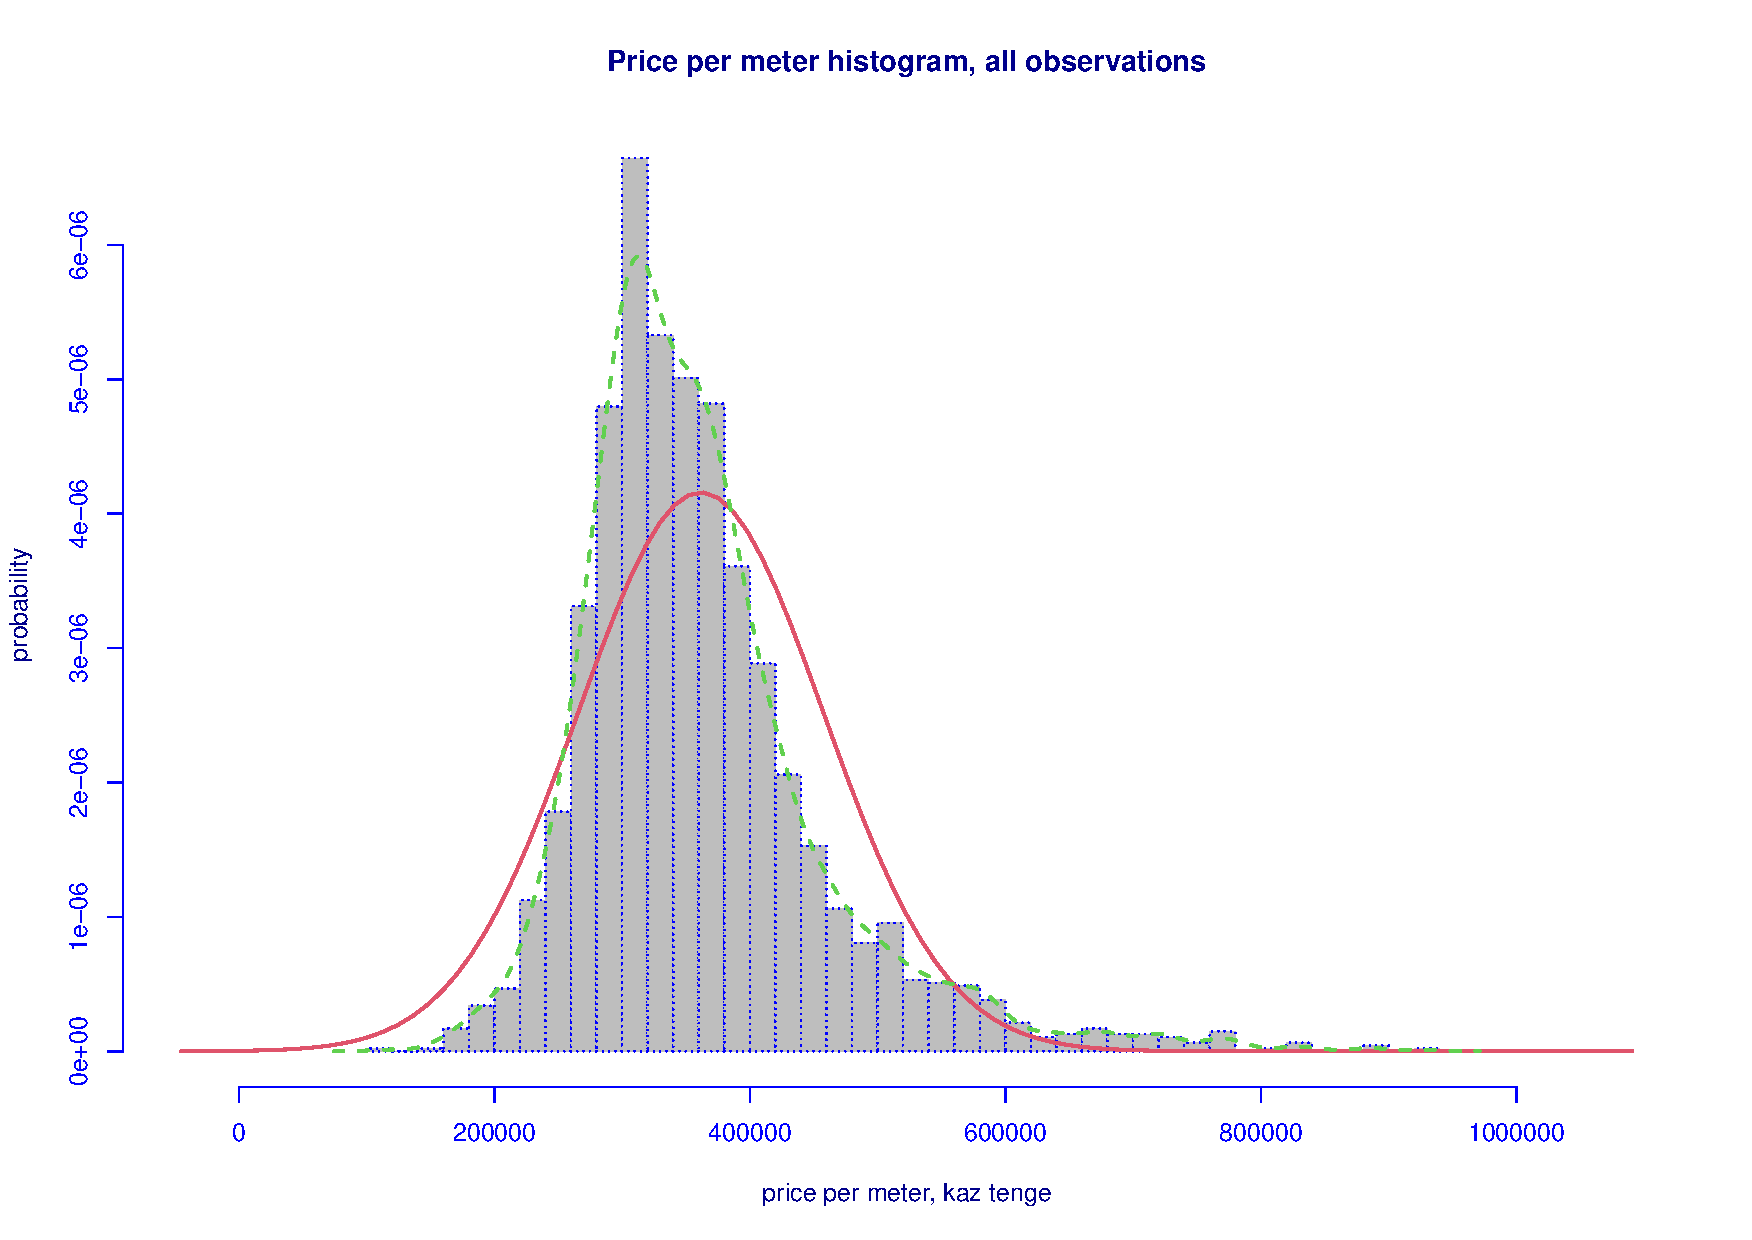
\includegraphics[width=0.95\textwidth]{almaty-hist-all.pdf}
	\caption{Гистограмма цен предложения для~всех объектов, совмещённая с~кривой функции плотности эмпирического распределения, а~также кривой функции плотности теоретического нормального распределения.}
	\label{fig:almaty-hist-all-r}
\end{figure}
%
%
\begin{figure}[ht]
	\centering
	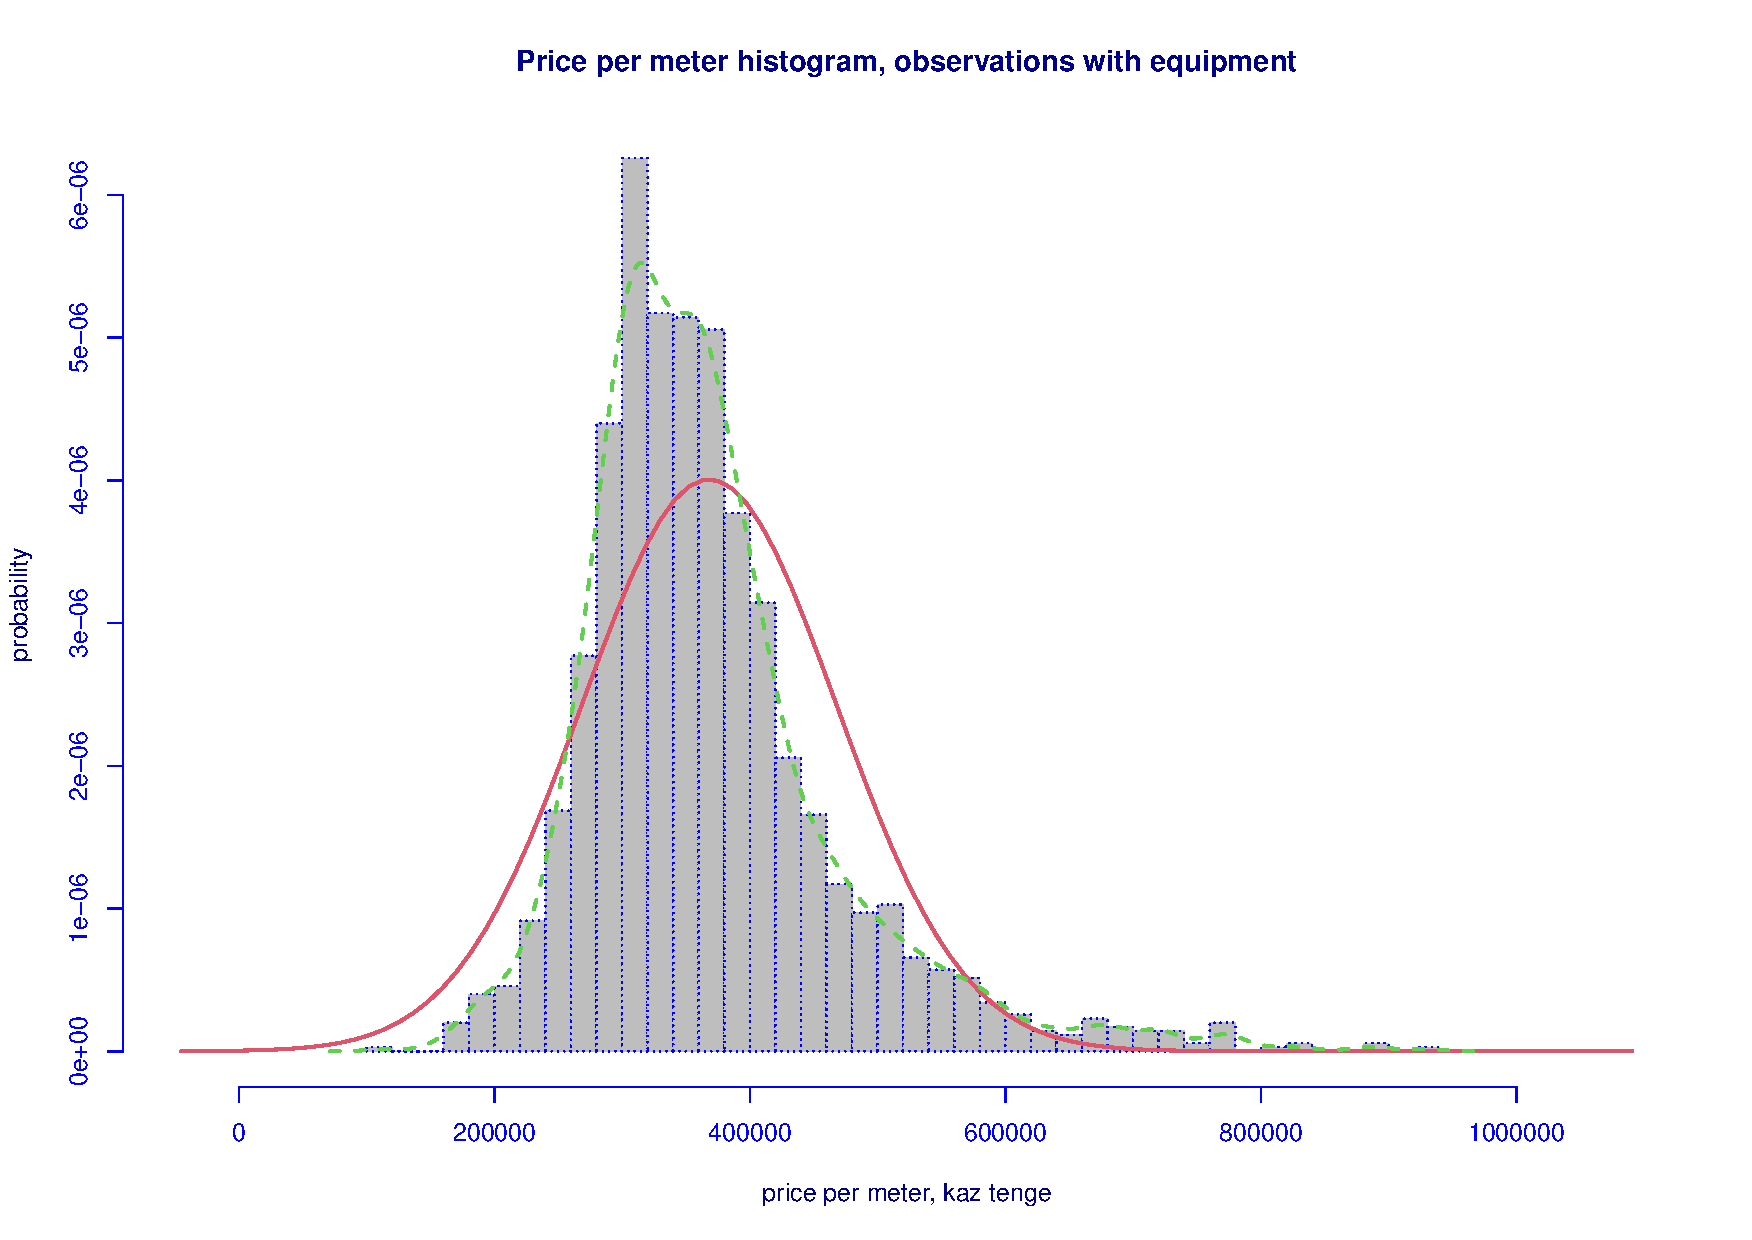
\includegraphics[width=0.95\textwidth]{almaty-hist-equiped.pdf}
	\caption{Гистограмма цен предложения для~объектов, предлагаемых к~продаже предлагаемых к~продаже совместно с~отделимыми улучшениями, совмещённая с~кривой функции плотности эмпирического распределения, а~также кривой функции плотности теоретического нормального распределения.}
	\label{fig:almaty-hist-equiped-r}
\end{figure}
%
%
\begin{figure}[ht]
	\centering
	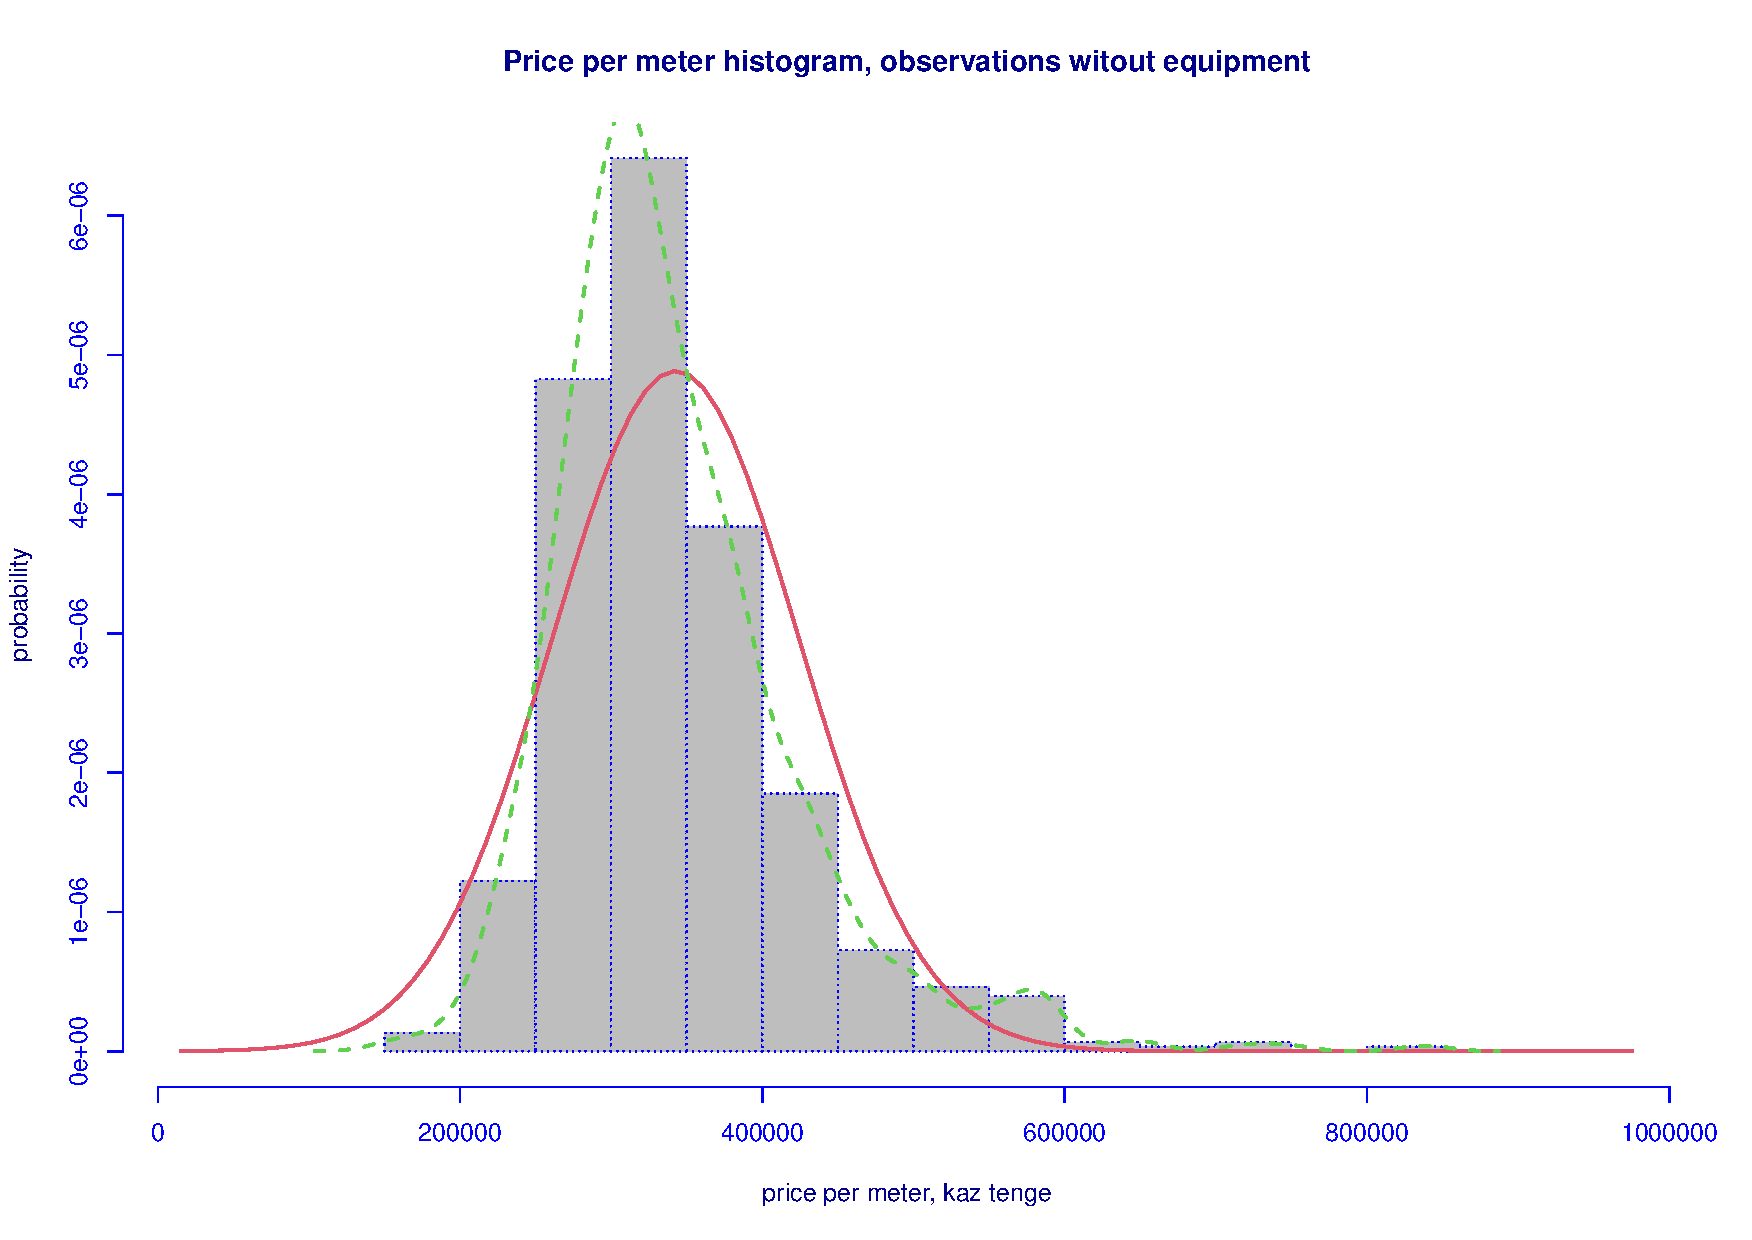
\includegraphics[width=0.95\textwidth]{almaty-hist-nequiped.pdf}
	\caption{Гистограмма цен предложения для~объектов, предлагаемых к~продаже без~отделимых улучшений, совмещённая с~кривой функции плотности эмпирического распределения, а~также кривой функции плотности теоретического нормального распределения.}
	\label{fig:almaty-hist-nequiped-r}
\end{figure}
%
\begin{table}[ht]
	\caption{Базовые описательные статистики наблюдений различных типов на~рынке города Алматы (единица "--- казахстанский тенге)}\label{tab:summaries-almaty-R}
	\centering
	\begin{tabular}{lllllllll}
		\hline
		Тип наблюдений&Min&1Q&Медиана&Среднее&3Q&Max\\
		\hline
		Все~наблюдения&117000&300000&344432&361554&400000&928571\\
		\hline
		Наблюдения без~отделимых улучшений&152542&291803&325581&342581&378788&838462\\
		\hline
		Наблюдения с~отделимыми улучшениями&117000&305446&350331&368113&406183&928571\\
		\hline
	\end{tabular}
\end{table}
%
\begin{figure}[ht]
	\centering
	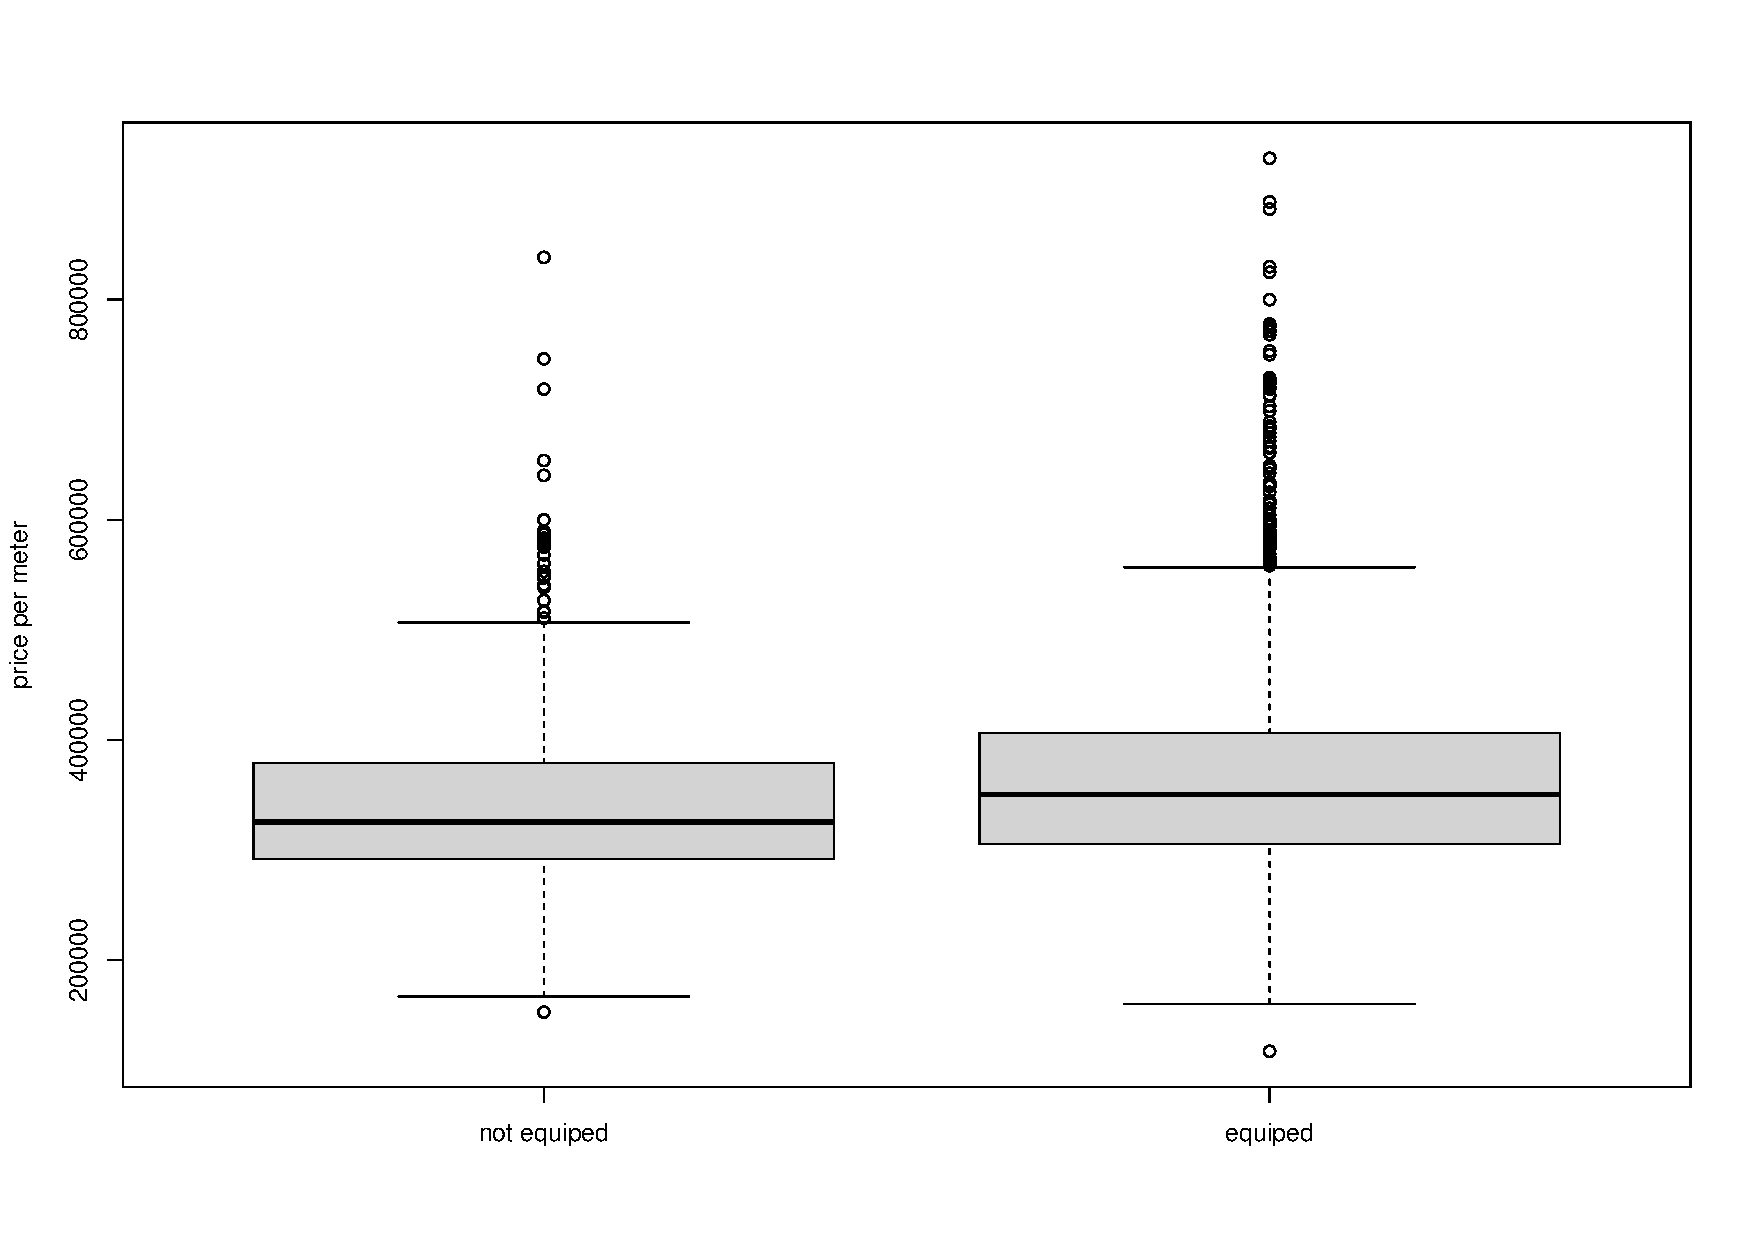
\includegraphics[width=0.95\textwidth]{almaty-boxplot.pdf}
	\caption{Диаграмма <<ящик с~усами для~рынка Алматы>>.}
	\label{fig:almaty-boxplot-r}
\end{figure}
%
\begin{lstlisting}[float, caption = Построение диграммы <<ящик с~усами>> для~рынка Алматы, firstnumber=1, label= lst:boxplot-R]
# plot boxplots
nequiped <- subset(almatyFlats, furniture == 0)
equiped <- subset(almatyFlats, furniture > 0)
boxplot(nequiped$price.m, equiped$price.m,
ylab = 'price per meter',
names =c('not equiped', 'equiped'))
rm(nequiped)
rm(equiped)
\end{lstlisting}
%

Следующий этап анализа заключается в~проверке нормальности распределения удельных цен предложений. Как~уже было сказано выше, язык~R обладает очень богатым набором инструментов. Существует множество библиотек, предлагающих в~общей сложности несколько десятков тестов. В~данной работе были применены следующие тесты:
\begin{itemize}
	\item критерий Шапиро"--~Уилка~\cite{Shapiro-Wilk-test};
	\item критерий Шапиро"--~Франчиа~\cite{Shapiro-Francia-test};
	\item критерий Андерсона"--~Дарлинга~\cite{Anderson-Darling-test};
	\item скорректированный критерий Харка"--~Бера~\cite{Jarque-Bera-test};
	\item критерий Колмогорова"--~Смирнова с~поправкой Лилиефорса~\cite{Liliefors-normality-test}.
\end{itemize}
Код для~проведения тестов для~объектов, продаваемых без~отделимых улучшений, приведён в~скрипте~\ref{lst:normality-tests-nequiped-R}, вместе с~ними "--- \ref{lst:normality-tests-equiped-R}.
Результаты тестов для~обеих групп сведены в~таблицу~\ref{tab:normality-tests-values-R}. Результаты всех тестов позволяют сделать однозначный вывод: распределения обеих подвыборок отличаются от~нормального, что~указывает на~необходимость применения непараметрических критериев.
%
\begin{lstlisting}[float, caption = Проведение тестов на~нормальность для~наблюдений без~отделимых улучшений, firstnumber=1, label= lst:normality-tests-nequiped-R]
# normality tests for non equipped observations
# Shapiro-Wilk test for normality
shapiro.test(almatyFlats$price.m[ which(almatyFlats$furniture == 0)])
# Shapiro-Francia test for normality
sf.test(almatyFlats$price.m[ which(almatyFlats$furniture == 0)])
# Anderson-Darling test for normality
ad.test(almatyFlats$price.m[ which(almatyFlats$furniture == 0)])
# Adjusted Jarque-Bera test for normality
ajb.norm.test(almatyFlats$price.m[ which(almatyFlats$furniture == 0)])
# Lilliefors (Kolmogorov-Smirnov) test for normality
lillie.test(almatyFlats$price.m[ which(almatyFlats$furniture == 0)])
\end{lstlisting}
%
\begin{lstlisting}[float, caption = Проведение тестов на~нормальность для~наблюдений с~отделимыми улучшениями, firstnumber=1, label= lst:normality-tests-equiped-R]
# normality tests for non equipped observations
# Shapiro-Wilk test for normality
shapiro.test(almatyFlats$price.m[ which(almatyFlats$furniture > 0)])
# Shapiro-Francia test for normality
sf.test(almatyFlats$price.m[ which(almatyFlats$furniture > 0)])
# Anderson-Darling test for normality
ad.test(almatyFlats$price.m[ which(almatyFlats$furniture > 0)])
# Adjusted Jarque-Bera test for normality
ajb.norm.test(almatyFlats$price.m[ which(almatyFlats$furniture > 0)])
# Lilliefors (Kolmogorov-Smirnov) test for normality
lillie.test(almatyFlats$price.m[ which(almatyFlats$furniture > 0)])
\end{lstlisting}
%

\begin{table}[ht]
	\caption{Результаты проведения тестов проверки данных по~г.~Алматы на~нормальность $({\textstyle \alpha=0.05})$}\label{tab:normality-tests-values-R}
	\centering
	\begin{tabular}{lll}
		\hline
		Тест&Без отделимых улучшений&С отделимыми улучшениями\\
		\hline
		Шапиро"--~Уилка:&\ref{lst:normality-tests-nequiped-R}&\ref{lst:normality-tests-equiped-R}\\
		статистика критерия~(W)&0.9&0.9\\
		p-значение&<2e-16&<2e-16\\
		H0&отклоняется&отклоняется\\
		\hline
		Шапиро"--~Франчиа:&\ref{lst:normality-tests-nequiped-R}&\ref{lst:normality-tests-equiped-R}\\
		статистика критерия~(W)&0.9&0.9\\
		p-значение&<2e-16&<2e-16\\
		H0&отклоняется&отклоняется\\
		\hline
		Андерсона"--~Дарлинга&\ref{lst:normality-tests-nequiped-R}&\ref{lst:normality-tests-equiped-R}\\
		статистика критерия~(A)&13&42\\
		p-значение&<2e-16&<2e-16\\
		H0&отклоняется&отклоняется\\
		\hline
		Жарка"--~Бера (скорр.)&\ref{lst:normality-tests-nequiped-R}&\ref{lst:normality-tests-equiped-R}\\
		статистика критерия~(AJB)&757&1720\\
		p-значение&<2e-16&<2e-16\\
		H0&отклоняется&отклоняется\\
		\hline
		Лиллиефорса (К-С)&\ref{lst:normality-tests-nequiped-R}&\ref{lst:normality-tests-equiped-R}\\
		статистика критерия~(D)&0.1&0.1\\
		p-значение&<2e-16&<2e-16\\
		H0&отклоняется&отклоняется\\
		\hline
		Итоговый вывод:&&\\
		H0&отклоняется&отклоняется\\
		\hline
	\end{tabular}
\end{table}

Для~проведения U-теста достаточно выполнить код, содержащийся в~скрипте~\ref{lst:U-test-R}. Результаты теста приведены в~таблице~\ref{tab:u-test-r-result}. На~основании полученного результата можно сделать вывод о~том, что~учёт фактора наличия неотделимых улучшений и~движимого имущества должен быть произведён.
%
\begin{lstlisting}[float, caption = Проведение U-теста для данных города Алматы, firstnumber=1, label= lst:U-test-R]
# perform Mann-Whitney U-test
wilcox.test(almatyFlats$price.m[ which(almatyFlats$furniture == 0)],
almatyFlats$price.m[ which(almatyFlats$furniture > 0)]) 
\end{lstlisting}
%
\begin{table}[ht]
	\caption{Результаты проведения U-теста для~данных Алматы$({\textstyle \alpha=0.05})$}\label{tab:u-test-r-result}
	\centering
	\begin{tabular}{ll}
		\hline
		Показатель&Значение\\
		\hline
		Статистика критерия&441360\\
		\hline
		p-значение&1e-09\\
		\hline
		Нулевая гипотеза (см.~таблицу~\ref{tab:nul-alt-hypothesis-almaty})&отклоняется\\
		\hline
	\end{tabular}
\end{table}
%

\clearpage

\chapter{Выводы}
В~данной работе были рассмотрены теоретические и~практические аспекты применения критерия Манна"--~Уитни"--~Уилкоксона в~повседневной практике оценщика. Данный тест может стать надёжным критерием проверки значимости тех~или~иных признаков объектов-аналогов, наблюдаемых на~открытом рынке. Самостоятельный анализ рыночных данных является лучшим и, вероятно, единственным подлинно доказательным инструментом оценщика, стремящегося создавать ценность для~заказчика, а~также новые знания о~рынках. Несмотря на~некоторый начальный порог входа, анализ данных средствами языков программирования является достаточно простым. Строго говоря, часть сделанных шагов является избыточной и~была сделана с~целью продемонстрировать малую часть возможностей языков Python и~R, а~также показать важность визуализации данных. Минимальный набор действий, необходимых для~проведения U-теста включает следующие этапы:
\begin{itemize}
	\item загрузка данных и~создание датафрейма;
	\item создание двух подвыборок на~основе значения изучаемого признака;
	\item проведение тестов на~нормальность распределений (в~большинстве случаев достаточно проведения теста Шапиро"--~Франчиа либо К2~Д'Агостино);
	\item проведение U-теста.
\end{itemize}
С~учётом наличия готовых скриптов проведение теста занимает всего несколько минут.

Конечно~же наука не~стоит на~месте.

В~завершение материала хочется дать следующую рекомендацию: современному оценщику в~первую очередь необходимо изучать Python: скорее всего, его~инструменты исчерпывающе закроют все~потребности по~анализу данных. В~случае стремления к~совершенству и~наличия желания быть на~уровень выше, знание R может помочь в~решении особенно сложных и~нетривиальных задач. Впрочем, существуют и~\href{https://habr.com/ru/post/670250/}{альтернативные мнения}~\cite{Habr:Python-or-R}. Эпоха массового применения методов машинного обучения и~математической статистики только начинается, и~сейчас сложно предсказать, какие средства станут стандартом оценщика через 5 или~10~лет.
\clearpage
\printbibliography[title=Источники информации]

\end{document}
